\documentclass[a4paper,USenglish]{tex/lipics-v2016}
\usepackage{stmaryrd}
\usepackage{xspace,listings,url,framed,amssymb,
            mathpartir,hyperref,doi, mathtools,wrapfig,
            stmaryrd, graphicx, tikz, colortbl, xparse, etoolbox,
            pgffor, makecell, microtype}
\usepackage[customcolors,norndcorners]{hf-tikz}
\usetikzlibrary{arrows}
\usetikzlibrary{shapes.geometric}
\usetikzlibrary{shapes.multipart}
\usetikzlibrary{positioning}
\usetikzlibrary{calc}
\usetikzlibrary{backgrounds}
\usepackage[inline]{enumitem}
\usepackage{epigraph}
\setlength{\epigraphrule}{0pt}
\renewcommand*{\textflush}{flushright}
\setlength{\epigraphwidth}{4in}
\newcommand{\code}[1]{{\tt #1}\xspace}
\newcommand{\FZ}[1]{\textbf{FZ: #1}}
%% Formatting
\newcommand{\M}[1]{\ensuremath{#1}\xspace}
\newcommand{\xt}[1]{{\sf{#1}}}
\newcommand{\bt}[1]{\xt{\bf #1}}
\renewcommand{\b}[1]{\M{\overline{#1}}}
\newcommand{\Mxt}[1]{\M{\xt{#1}}}
\newcommand{\Mbt}[1]{\M{\bt{#1}}}

%% Variables
\newcommand{\x}   {\Mxt x}
\newcommand{\e}   {\Mxt e}
\newcommand{\m}   {\Mxt m}
\newcommand{\s}   {\M{\sigma}}
\renewcommand{\t} {\Mxt t}
\renewcommand{\a} {\Mxt a}
\newcommand{\K}   {\Mxt K}
\renewcommand{\k} {\Mxt k}
\newcommand{\Kp}  {{\Mxt{K'}}}
\newcommand{\ep}  {{{\Mxt{e'}}}}
\renewcommand{\sp}{{{\M{\s'}}}}
\newcommand{\ap}  {\M{\a'}}
\newcommand{\tp}  {\M{ \t'}}
\newcommand{\C}   {\Mxt C}
\newcommand{\Cp}  {\Mxt{C'}}
\newcommand{\fd}  {\Mxt{fd}}
\newcommand{\md}  {\Mxt{md}}
\newcommand{\mt}  {\Mxt{mt}}
\newcommand{\f}   {\Mxt f}
\newcommand{\E}   {\M \Gamma}
\newcommand{\any} {\M{\star}}
\newcommand{\this}{\Mxt{this}}
\newcommand{\none}{\M{\cdot}}
\newcommand{\D}   {\Mxt D}

\newcommand{\Get}[2]   {\M{#1.#2()}}
\newcommand{\Set}[3]   {\M{#1.#2(#3)}}
\newcommand{\Call}[3]  {\M{#1.#2(#3)}}

\newcommand{\DynGet}[2]   {\M{#1@#2()}}
\newcommand{\DynSet}[3]   {\M{#1@#2(#3)}}
\newcommand{\DynCall}[3]  {\M{#1@#2(#3)}}

\newcommand{\New}[2]   {\M{\new\;#1(#2)}}
\newcommand{\wCast}[2] {\M{<{#1}>\;{#2}}}
\newcommand{\mCast}[2] {\M{\prec #1 \succ #2}}
\newcommand{\tCast}[2] {\M{\triangleleft\; #1 \triangleright #2}}
\newcommand{\cCast}[2] {\M{\blacktriangleleft #1 \blacktriangleright #2}}
\newcommand{\new}      {\M{\bt{new}}}
\newcommand{\HT}[2]    {\M{{#1}\!:{#2}}}
\newcommand{\Mdef}[5]  {\M{ \HT{ #1( \HT{#2}{#3})}{#4}~\{\,{#5}\,\}}}
\newcommand{\Mdefz}[3] {\M{ \HT{ #1()}{#2}~\{\,{#3}\,\}}}
\newcommand{\Ctx}[1]   {\M{\xt{E}[#1]}}
\newcommand{\Obj}[2]   { \M{ #2\{#1\}}}
\newcommand{\obj}[2]   { \M{ #1\{#2\}}}
\newcommand{\alloc}[4] {\M{#1\;#2  = \xt{alloc}(#3, #4)}}
\newcommand{\cast}[8]  {\M{#6\;#7\;#8=\xtns{#5 cast}(#1, #2, #3, #4)}}
\newcommand{\Alt}[1]   { &\B #1 \\}
\newcommand{\B}        {\M{~|~}}
\newcommand{\bang}     {\M{\xt{!}}}

\newcommand{\dispatch}[5] {\M{#1\;#2 = \xt{disp}(#3,#4,#5)}}
\newcommand{\readfield}[4]{\M{#1 = \xt{read}(#2,#3,#4)}}
\newcommand{\setfield}[5] {\M{#1 = \xt{write}(#2,#3,#4,#5)}}
\newcommand{\Reduce}[6]   {\M{{#1}~{#2}~{#3} \rightarrow {#4}~{#5}~{#6}}}
\newcommand{\ReduceA}[6]  {\M{#1~#2~#3 } & \M{\rightarrow #4~#5~#6}}
\newcommand{\Class}[3]    {\M{\bt{class}\;#1\,\{\,#2~#3\,\}}}
\newcommand{\Ftype}[2]    {\M{ \HT{#1}{#2} }}
\newcommand{\Mtype}[3]    {\M{ \HT{#1(#2)}{#3}}}
\newcommand{\Type}[1]     {\M{\{#1\}}}

\newcommand{\opdef}[2]    {\framebox[1.1\width]{#1} ~ #2\\}
\newcommand{\Heap}[2]     {\M{ #1[#2] }}
\newcommand{\Bind}[2]     {\M{#1 \mapsto #2}}

\newcommand{\Sub}{\M{<:}}
\newcommand{\ConsSub}{\M{\lesssim}}

\newcommand{\CondRule}[3]{ #3 &~{\emph{if}} #2 \\}
\newcommand{\EnvType}[3]{ \M{#1 \vdash #2 : #3}}
\newcommand{\Es}{\E ~\s}
\newcommand{\tw}[1]{\M{\xt{typed}(#1)}}
\newcommand{\IRule}[3]{\inferrule*[lab={\tiny #1}]{#2}{#3}}
\newcommand{\HasType}[3]{ \M{#1 (#2) = #3}}
\newcommand{\inc}{\M{\in}}
\newcommand{\wrapper}[1]{\M{\xt{wrap}(#1)}}
\newcommand{\xtns}[1]{{\sf{#1}}}
\newcommand{\utw}[1]{\M{\xt{untyped}(#1)}}
\newcommand{\meet}[2]{#1\sqcap #2}
\newcommand{\spec}[1]{\M{\xt{spec}(#1)}}

\newcommand{\castfn}[4]{\text{cast}(#1,#2,#3,#4)}
\newcommand{\GenCast}[4]{#1 \vdash #2 \hookrightarrow #3 \Uparrow #4 }
\newcommand{\AnaCast}[4]{#1 \vdash #2 \Downarrow #4 \hookrightarrow #3}
\newcommand{\TransClass}[2]{\M{ #1 \rightharpoonup #2 }}
\newcommand{\inv}[2]{\xt{invoke}(#1, #2)}

\newcommand{\III}{}
\III{

\newcommand{\n}{\M{\xt{n}}}
\renewcommand{\d}{\M{\xt{d}}}
\renewcommand{\r}{\M{\xt{r}}}
\newcommand{\fb}{\M{\xt{f!}}}
\renewcommand{\c}{\M{\xt{c}}}
\renewcommand{\d}{\M{\xt{d}}}
\newcommand{\T}{\M{\xt T}}
\newcommand{\cbp}[1]{\M{ \b{\C_{#1}}}}
\renewcommand{\mp}[1]{\M{ \m_{#1} }}
\newcommand{\class}{\M{\bt{class}}}
\newcommand{\SMdef}[5]{\M{ \HT { #1!( \HT{#2}{#3})}{#4}= {#5}}}
\newcommand{\GMdef}[3]{\M{ \HT { #1()}{#2}={#3}}}
\newcommand{\Fdef}[3]{\M{ \HT{#1}{#2}={#3} }}
\newcommand{\notdispatch}[5]{\M{#1,#2 \not = \xt{dispatch}(#3,#4,#5)}}
\newcommand{\NoCondRule}[2]{ #2 &       \\}
\newcommand{\Update}[3]{\M{#1[ #2 := #3]}}
\newcommand{\NotSub}{\M{\not<:}}
\newcommand{\classofis}[2]{\M{\xt{classof}(#1)=#2}}
\newcommand{\typeofis}[3]{\M{\xt{typeof}(#1,#2)=#3}}
\newcommand{\classof}[1]{\M{\xt{classof}(#1)}}
\newcommand{\typeof}[2]{\M{\xt{typeof}(#1,#2)}}
\newcommand{\Sel}[2]{\M{#1(#2)}}
\newcommand{\TransExp}[4]{\M{ #1 \vdash #2 \hookrightarrow #3 : #4 }}
\newcommand{\mdp}[1]{\M{\md_{#1}}}
\newcommand{\setter}[1]{\M{\xt{set}(#1)}}
\newcommand{\getter}[1]{\M{\xt{get}(#1)}}
\newcommand{\dynamic}[1]{\M{\xt{dyn}(#1)}}
\newcommand{\invoke}[1]{\M{\xt{inv}(#1)}}
\newcommand{\Dyn}[1]{\M{#1^{\any} }}
\newcommand{\casts}[1]{\M{\xt{casts}(#1)}}
\newcommand{\fcast}[1]{\M{\xt{translate}(#1)}}
\newcommand{\proxy}[1]{\M{\xt{proxy}(#1)}}
%\newtheorem{definition}{Definition}
%\newtheorem{thm}{Theorem}
\newcommand{\WF}[1]{\ensuremath{\xt{WF}(#1)}\xspace}
\newcommand{\Weak}{\text{\small?}\hspace{0.1em}}
\newcommand{\WType}[1]{\Weak\Type{#1}}


\newcommand{\stcons}[2]{#1\lesssim #2}
\newcommand{\refine}[2]{#1\vartriangleright #2}
\newcommand{\inscast}[1]{\M{\llbracket #1 \rrbracket_{\xt{ins}}}}
\newcommand{\adapt}[1]{\M{\llbracket #1 \rrbracket_{\xt{adapt}}}}

\newcommand{\p}{\xt{p}}
\newcommand{\cb}{\b{\C}}
\newcommand{\typed}[1]{\text{typed}(#1)}
\newcommand{\untyped}[1]{\text{untyped}(#1)}
\newcommand{\includecode}[2][c]{\lstinputlisting[caption=#2, escapechar=, style=custom#1]{#2}<!---->}

\newcommand{\ESub}[3]{#1 \vdash #2 \leq #3}
\newcommand{\Vect}[3]{\text{Vec}(#1,#2,#3)}
\newcommand{\tv}{\xt{v}}
\newcommand{\ts}{\xt{ts}}
\newcommand{\MetaSub}[2]{\xtns{Sub}(#1,#2)}

}

\definecolor{Gray}{gray}{0.9}
\definecolor{vlightgray}{gray}{0.93}
\pagestyle{headings} 

\lstdefinelanguage{JavaScript}{
  keywords={typeof,new,true,false,instanceof,catch,function,return,null, 
    catch, switch, var, if, in, while, do, else, case, break},
  keywordstyle=\color{darkgray},
  ndkeywords={class,def,interface,export,boolean,throw,extends,implements,import,this},
  ndkeywordstyle=\color{darkgray}\bfseries,
  identifierstyle=\color{black},
  sensitive=false,  comment=[l]{//},  morecomment=[s]{/*}{*/},
  commentstyle=\color{gray}\ttfamily,  stringstyle=\color{gray}\ttfamily,
  morestring=[b]',  morestring=[b]",
  %backgroundcolor=\color{vlightgray},
  aboveskip=\medskipamount, %0em,
  belowskip=\medskipamount, %0em
  escapeinside={(*@}{@*)}
}
\lstset{
  language=JavaScript,  extendedchars=true,  basicstyle=\small\ttfamily,
  showstringspaces=false,   showspaces=false,  numberstyle=\small,
  numbersep=9pt,  tabsize=2, breaklines=true,  showtabs=false, captionpos=b
}

\begin{document}
\title{KafKa: A Common Framework for Gradual Typing of Objects}
\titlerunning{Gradual typing of objects}

\author[1]{Benjamin Chung}
\author[2]{Paley Li}
\author[3]{Jan Vitek}
\affil[1]{Northeastern University}
\affil[2]{CVUT Prague}
\affil[3]{Northeastern University}
\authorrunning{B.chung, P. Li, J. Vitek} %mandatory. First: Use abbreviated first/middle names. Second (only in severe cases): Use first author plus 'et. al.'


\Copyright{John Q. Open and Joan R. Access}%mandatory, please use full first names. LIPIcs license is "CC-BY";  http://creativecommons.org/licenses/by/3.0/

\subjclass{Dummy classification -- please refer to \url{http://www.acm.org/about/class/ccs98-html}}% mandatory: Please choose ACM 1998 classifications from http://www.acm.org/about/class/ccs98-html . E.g., cite as "F.1.1 Models of Computation". 
\keywords{Dummy keyword -- please provide 1--5 keywords}% mandatory: Please provide 1-5 keywords
% Author macros::end %%%%%%%%%%%%%%%%%%%%%%%%%%%%%%%%%%%%%%%%%%%%%%%%%

%Editor-only macros:: begin (do not touch as author)%%%%%%%%%%%%%%%%%%%%%%%%%%%%%%%%%%
\EventEditors{John Q. Open and Joan R. Acces}
\EventNoEds{2}
\EventLongTitle{42nd Conference on Very Important Topics (CVIT 2016)}
\EventShortTitle{CVIT 2016}
\EventAcronym{CVIT}
\EventYear{2016}
\EventDate{December 24--27, 2016}
\EventLocation{Little Whinging, United Kingdom}
\EventLogo{}
\SeriesVolume{42}
\ArticleNo{23}
% Editor-only macros::end %%%%%%%%%%%%%%%%%%%%%%%%%%%%%%%%%%%%%%%%%%%%%%%


\maketitle

\begin{abstract}
The enduring popularity of dynamically typed languages has motivated
research on \emph{gradual type systems} to allow developers to annotate
legacy dynamic code piecemeal. Type soundness for a program which contains a
mixture of typed and untyped code cannot mean the traditional absence of
errors. While some errors will caught at type checking time, others can only
be caught as the program executes. After a decade of research it is clear
that the combination of mutable state, aliasing and subtyping presents
challenges to gradual type systems.  We introduce \kafka, a class-based
object calculus with a static type system, dynamic method dispatch,
transparent wrappers and dynamic class generation. \kafka was designed as a
common framework for expressing the semantics of various gradually typed
object-oriented languages. We demonstrate the usefulness by translating
idealizations of four different gradually typed language languages into the
calculus and discuss the implications of their respective designs.
\end{abstract}

\section{Introduction}

%\epigraph{\small\it ``Because half the problem is seeing the problem''}
%\vspace{-5mm}

\noindent A decade ago Siek and Taha~\cite{SiekTaha07} presented a gradual
type system for a variant of Abadi and Cardelli's object-based
calculus~\cite{cardelli:1996:theory-of-objects}. Their system featured a
dynamic type, denoted \any, and a subtype relation that combined structural
subtyping with a consistency relation between terms that only differ in
dynamic type annotations.  Soundness at the boundaries between typed and
untyped code is ensured by inserting casts following in their earlier work
for functional languages~\cite{SiekTaha06}.

A decade later, practical realizations of Siek and Taha's elegant idea have
proved elusive. One potential reason may be that the original paper did not
consider state. The combination of mutable state, aliasing and subtyping
prevalent in object-oriented languages complicates enforcement strategies,
as one must consider situations where an object is being accessed and
mutated at different types. While solutions have been proposed, their
performance implications are a source of concern.

This paper explores the design space of gradual type systems for
object-oriented languages by studying four approaches, each with markedly
different characteristics in terms of errors and overheads.  These
approaches are representative of most languages with implementations
available in open source. The \emph{optional} approach, chosen by
TypeScript, Dart, and Hack, amounts to static type-checking followed by
erasure. Optional types do not impact performance, but fail to catch cases
when erroneous values flow from dynamically typed code to statically typed
code.  The \emph{concrete} approach, used in C\#, Thorn, and StrongScript,
combines optional types, runtime type casts and traditional static
typing. This approach allows statically typed code to execute at native
speed, but is somewhat more restrictive in terms of which values can cross
type boundaries, as they must satisfy a runtime type cast. The
\emph{behavioral} approach, followed by Typed Racket, Gradualtalk and
Reticulated Python, monitors values to ensure that they behave in accordance
to their assigned types. This approach is the closest to the Siek and Taha
proposal, but also the approach with the most significant performance
overheads. Finally, the \emph{transient} approach, specific to the
Reticulated Python language, lies between concrete and behavioral; it adds
type casts but does so only for the top-level of data structures. The cast
insertion strategy is related to the tests performed by behavioral types
except transient, that instruments code and not values.

While the software engineering benefits of the different approaches are being
debated, it is worthwhile to observe that the definition of type error is also
open for debate.  Each of the approaches will catch different errors.
Specifically, our work demonstrates with a litmus test consisting of three
simple programs that it is possible to distinguish the type systems. These
three programs can be expressed in all four approaches (source code is
included in appendix) and the programs are statically well typed for all
languages. The programs are ``correct'' in the sense that in an untyped
language they run to completion without error. In the gradual type systems,
they display different errors.  The significance of this observation is that
there are still design questions that must be resolved. For instance, consider
a call of the form \code{x.m()} for where the typed call, with the concrete
approach, this statement is guaranteed to succeed, with an optional approach
the call to \code{m} may fail because \code{x} lacks method \code{m}, while in
behavioral the call will succeed, but a failure may occur upon return if the
returned value does not have the expected methods.

This paper introduces a core calculus for evaluating gradual type systems
for object-oriented languages. The calculus, \kafka, is a statically typed
class-based object calculus with mutable state expressly designed designed
to support different gradual type systems. The calculus has a number of
features specifically for that purpose. It has two kinds of type casts.
Structural casts, \SubCast\t\a, check if the object referenced by \a is a
subtype of type \t.  Behavioral casts, \BehCast\t\a, create wrappers that
enforce that the object referenced by \a behaves as if it was of type \t.
To do this, the calculus support runtime generation of a classes and
transparent wrappers.  The \kafka type system has two kinds of types;
classes and the dynamic type \any.  More technically, \kafka has two kinds
of method calls, statically resolved calls, \KCall\a\m\x\t\tp, and
dynamically resolved ones, \DynCall\a\m\x, where a soundness guarantee is 
provided for static calls, but not for dynamically resolved ones.

This paper presents a semantics for \kafka and reports on a mechanized proof
of soundness for \kafka in Coq inclusive of its casts and of the runtime
class generation needed to implement them.  We completed a proof-of-concept
implementation of the calculus on top of the .NET virtual machine to
demonstrate that this design matches the features available in commercial
system. The only challenge in that implementation was to support structural
subtyping which is required by behavioral and transient, neither approach is
sensible in nominal type system.

Gradually typed languages can be represented as translations from source
terms into \kafka term.  These translations make explicit which of the
underlying type system's guarantees can be relied upon statically, and where
dynamism is really required. Part of our contribution are the four
translations, each taking a gradually typed expression \HT\e\T in a source
language implementing one of the above mentioned approaches and returning
the corresponding \kafka term. The translation of a term entails translating
the classes needed to evaluate it.  The translations allows us to study
where program can get stuck in the different systems.  With gradual types,
an expression \Call\x\m\e, where \x is declared to be of class \C, can have
significantly different behavior depending on choices made while designing
the type system. We believe that expressing the semantics of gradually typed
object-oriented languages as translations into a core illuminates the
difference and similarities between designs.


\section{Background}

%\epigraph{\small\it ``If you know the enemy and know yourself...''}
%\vspace{-5mm}

\noindent The intellectual lineage of gradual types can be traced back to
attempts to add types to Smalltalk and LISP. A highlight on the Smalltalk
side is the Strongtalk optional type system~\cite{Bracha93}, which led to
Bracha's notion of pluggable types~\cite{pluggabletypes}. For him, types
exist solely to catch errors at compile-time, never affecting the runtime
behavior of programs. The rationale is that types are an add-on that can be
turned off without affecting semantics.  In the term of Richards~\emph{et
  al.}~\cite{ecoop15}, an optional type system is \emph{trace preserving}, a
if when term \e reduces to value \a, adding type annotations will never
cause \e to get stuck. This property is valuable to developers as type
annotations will not introduce errors (or affect performance).  Optional
type systems in wide use include Hack~\cite{hack13}, TypeScript~\cite{BAT14}
and Dart~\cite{dart13}.

On the functional side, the ancestry is dominated by the work of Felleisen
and his students.  The Typed Scheme~\cite{tf-popl08} design that later
became Typed Racket is influenced by the authors' earlier work on
higher-order contracts~\cite{ff-icfp02}. Typed Racket was envisioned as a
vehicle for teaching programming, thus being able to explain the source of
errors was an important design consideration. Another consideration was to
prevent surprises for beginning users, thus the value held in a variable
annotated as a \C should always behave as a \C. To aid debugging, any
departure from the expected behavior of an object, as defined by its
behavioral type, must be reported at the first discrepancy.  Whenever a value
crosses a boundary between typed and untyped code, it is wrapped in a
contract that monitors its behavior. This ensures that mutable values
remains consistent with their declared type and functions respect their
declared interface. When a value misbehaves, blame can be assigned to a
boundary. The granularity of typing is the module, thus a module is either
entirely typed or entirely untyped. 


Siek and Taha coined the term gradual typing in~\cite{SiekTaha06} as ``any
type system that allows programmers to control the degree of static checking
for a program by choosing to annotate function parameters with types, or
not.'' Their contribution was a formalization of the idea in a lambda
calculus with references and a proof of soundness. They defined the type
consistency relation $\t \sim \tp$ which states that types that agree on
non-\any positions are compatible.  In~\cite{SiekTaha07} the authors
extended their result to a stateless object calculus and combined
consistency with structural subtyping, but extending this approach to
mutable objects proved challenging.  Reticulated Python~\cite{siek14} is a
compromise between soundness and efficiency.  The language has three modes:
the \emph{guarded} mode behaves as Racket with contracts applied to values.
The \emph{transient} mode performs shallow checks on reads and returns, only
validating if the value obtained has matching method names.  The
\emph{monotonic} mode is fundamentally different. Under the monotonic
semantics, a cast updates the type of an object in place by replacing some
of the occurrences of \any with more specific types, which can then
propagate recursively through the heap until a fixed point is
reached.\footnote{A previous version of this paper provided a translation
  for monotonic. We removed it for space reason and because the authors
  of Reticulated Python seem to have abandoned the approach.}

Other noteworthy systems include Gradualtalk~\cite{GS13}, C\#
4.0~\cite{Bierman10}, Thorn~\cite{oopsla09}, and
StrongScript~\cite{ecoop15}. Gradualtalk is a variant of Smalltalk with
Felleisen-style contracts and mostly nominal type equivalence (structural
equivalence can be specified on demand, but it is, in practice, rarely
used). C\# 4.0 adds the type {\sf dynamic} to C\# and dynamically resolved
method invocation.  C\# has thus a dynamic sublanguage that allows
developers to write unchecked code, working alongside a strongly typed
sublanguage in which values are guaranteed to be of their declared type.
The implementation replaces \any by the type {\tt object} and adds casts
where needed.  Thorn and StrongScript extend the C\# approach with the
addition of optional types (called {\em like types} in Thorn).  Thorn is
implemented by translation to the JVM. StrongScript translate to an extended
version of V8. The presence of concrete types means that the compiler can
optimize code (unbox data and in-line methods) and programmers are
guaranteed that type errors will not occur within concretely typed code.


\newcommand{\rot}[1]{\rotatebox{80}{#1}\hspace{-10px}}
\newcommand{\X}{\EM{\bullet}}
\newcommand{\XX}{\EM{\bullet^{(2)}}}
\newcommand{\XY}{\EM{\bullet^{(1)}}}

\begin{figure}[!t]
  \center
  {\footnotesize
\begin{tabular}{r|lllllllllllllr}
 & & \rot{Nominal}
  & \rot{Optional types}
  & \rot{Concrete types}
  & \rot{Behavioral types}
  & \rot{Class based}
  & \rot{First-class Class}
  & \rot{Soundness claim}
  & \rot{Unboxed prim.}
  & \rot{Subtype cast}
  & \rot{Shallow cast}
  & \rot{Generative cast}
  & \rot{Blame}
  & \rot{Pathologies}
  \\
Dart         &&\X &\X &   &   &\X &   &    &    &\X &   &   &   &  - 
\\\hline
Hack         &&\X &\X &   &   &\X &   &    &    &\X &   &   &   &  -  
\\\hline
TypeScript   &&   &\X &   &   &\X &   &    &    &   &   &   &   &  -  
\\\hline
C\#          &&\X &\X &\X &   &\X &   &\XX & \X &\X &   &   &   &  -  
\\\hline
Thorn        &&\X &\X &\X &   &\X &   &\XX & \X &\X &   &   &   & 0.8x
\\\hline
StrongScript &&\X &\X &\X &\X &\X &   &\XX &    &\X &   &\X &   & 1.1x   
\\\hline
Gradualtalk  &&\XY&   &   &\X &\X &   & \X &    &   &   &\X &\X &  5x
\\\hline
Typed Racket &&   &   &   &\X &\X &\X &\X  &    &   &\X &\X &\X & 121x 
\\\hline
Reticulated Python    \\
\it Transient&&   &\X &   &   & \X &  & \X &    &   &\X &   &\X & 10x \\
\it Monotonic&&   &   &   &\X & \X &  & \X &    &   &   &\X &\X &  27x\\
\it Guarded  &&   &   &   &\X & \X &  & \X &    &   &   &\X &\X &  21x\\
\end{tabular}}
  \caption{Overview of implemented gradual type systems. (1) Gradualtalk has
    optional structural constraints. (2) Concretely typed expressions are
    sound in C\#, Thorn and StrongScript.}\label{over}
\end{figure}

\figref{over} reviews gradual type systems with publicly available
implementations. All languages here are class-based, except TypeScript which
has both classes and plain JavaScript objects. That choice does not appear
to be crucial to the approach, but since type declarations are needed,
classes are an obvious way to introduce them.  Most languages base subtyping
on explicit name-based subtype declarations (nominal subtyping, rather than
on structural similarities.  TypeScript uses structural subtyping, but does
not implement a runtime check for it.  Anecdotal evidence suggests that
structural subtyping is rarely needed in TypeScript~\cite{ecoop15}, and in
fact, StrongScript extends TypeScript changing subtyping back to nominal for
improved performance. While nominal subtyping leads to more efficient type
casts, the consistency relation used in Reticulated Python is fundamentally
structural, it would be nonsensical to use it in a nominal
system.\footnote{Consistency relates classes that differ in the number of
  occurrences of \any in their type signature and not whether they are
  declared to extend one another. There is no clear way to have consistency
  and nominal subtyping in the same context.}  For Racket, the heavy use of
first-class classes and class generation naturally leads to structural
subtyping as many of the classes being manipulated have no names and arise
during computation.

Optional types are the default execution mode for Dart, Hack and TypeScript.
Transient Reticulated Python is, in some senses, optionally typed as any
value can flow into a variable regardless of its type annotation, leading to
its ``open world'' soundness guarantee~\cite{siek14}.  In Thorn and C\#,
primitives are concretely typed; they can be unboxed without tagging.  The
choice of casts follows from other design decisions. Languages with concrete
types naturally tend to use subtype casts to establish the type of
values. For nominal systems, there are highly optimized algorithms. Shallow
casts are casts that only check the presence of methods, but not their
signature. These are used by Racket and Python to ensure some basic form of
type conformance. Behavioral casts are used when information such as a type
or a blame label must be associated with a reference or an object.

Blame assignment is a topic of investigation in its own right. Anecdotal
evidence suggests that the context provided by blame helps developers
pinpoint the provenance of errors. A fitting analogy are the stack traces
printed by Java when a program terminates abruptly. Developers working in,
e.g, C++ must run their program in a debugger to obtain the same
information. Stack traces have little runtime cost because they piggyback on
precise exceptions. Recording blame has a cost, but no data exists on its
performance impact. We do not consider blame further in this paper.

The last column of \figref{over} lists self-reported performance
pathologies.  These numbers are not comparable as they refer to different
programs and different configurations of type annotations. They are not
worst case scenarios either; most languages lack a sufficient corpus of code
to conduct a thorough evaluation.  Nevertheless, one can observe that for
optional types no overhead is expected, as the type annotations are erased
during compilation. Concrete types insert efficient casts, and lead to code
that can be optimized.  The performance of the transient semantics for
Reticulated Python is a worst case scenario for concrete types -- i.e. there
is a cast at almost every call. Finally, languages with behavioral casts
tend to suffer prohibitive slow downs in pathological cases. Compiler
optimizations for reducing these overheads are an active research topic.

%%%%%%%%%%%%%%%%%%%%%%%%%%%%%%%%%%%%%%%%%%%%%%%%%%%%%%%%%%%%%%%%%%%%%%%%%%%

\section{KafKa: A Core Calculus}\label{kafkacore}

%\epigraph{\hspace{-1cm}\small\it ``Aux chenilles du monde entier et aux papillons qu'elles renferment''}\vspace{-5mm}

\noindent \kafka is a class-based, statically typed, object-oriented
calculus. The distinctive features of the calculus are its support for both
typed and untyped method invocation, as well as dynamic class generation
through explicit class tables.  The features of \kafka are modeled on common
compilation targets for object-oriented language such as the JVM's Java
Bytecode or the .NET CLR's Common Intermediate Language, both of which are
typed intermediate languages with support for untyped method calls (through
reflection) and class generation (via dynamic loading). Our design is guided
by the intuition that the semantics of gradually-typed object-oriented
languages can be represented by translation to a common representation
through the introduction of \emph{casts} and \emph{wrappers}.

\begin{figure}[!h]\hrulefill

\vspace{4mm}

\small\begin{tabular}{@{}ll}

\begin{minipage}{7.2cm}\begin{tabular}{@{}l@{~}l@{}l@{}l@{}l@{}l@{}l@{}l}
\e\hspace{.1cm} ::= & \hspace{.2cm} \x        
   &\B \this         
   &\B \that      
   &\B \FRead\f  \\   
   & &
   &\B \FWrite\f\e 
   &\B \KCall\e\m\e\t\t \\
   & &   
   &\B \SubCast\t\e 
   &\B \BehCast\t\e \\
   & &   
   &\B \New\C{\e[1]..}  
   &\B \DynCall\e\m\e 
\end{tabular}\end{minipage}&
\begin{minipage}{2.4cm}\begin{tabular}{l@{~}l@{}l@{}l}
  \k &::= \Class \C {\fd[1]..}{\md[1]..} \\
 \md &::= ~ \Mdef\m\x\t\t\e \\ 
 \fd &::= ~ \Fdef\f\t \\ 
  \t &::= ~ \any  \B   \C  \\ 
\end{tabular}\end{minipage} 
\end{tabular}

\vspace{2mm}

\noindent\hrulefill\caption{\kafka Syntax.}\label{syn}
\end{figure}

\paragraph{Syntax}  
\kafka's syntax is given in \figref{syn}.  Types consist of class names \C,
\D and the dynamic type, written \any.  Class definitions have a class name
and sequences of field and method definitions,
\Class\C{\fd[1]..}{\md[1]..}. Field definitions consist of a field and its
type, \Fdef\f\t. Method definitions have (for simplicity) a single argument
and an expression, denoted \Mdef\m\x\t\t\e.  \kafka supports a limited form
of overloading, allowing both a typed implementation and an untyped
implementation for each method.  Fields are private to objects, and can be
accessed only from the object's scope; reading a field is denoted
\(\FRead\f\) and writing a field is denoted \(\FWrite\f\e \).  A statically
resolved call, denoted \KCall\e\m\ep\t\tp, is guaranteed to succeed as the
type system ensures that the expression \e will evaluate to an object of a
class which has a method \Mtype\m\t\tp. A dynamically resolved call,
\DynCall\e\m\ep, can get stuck if the object that \e evaluates to does not
have a method \Mtype\m\any\any.  We let meta-variables \x ranges over
variable names, \m and \f range over methods and fields respectively; \this
is a distinguished identifier representing a method receiver, while \that is
a distinguished field name that will be used in wrapper classes.  Providing
two different cast mechanisms is a key feature of the calculus.  The former,
the \emph{structural cast}, \(\SubCast\t\e\), denotes the usual subtype cast
that dynamically type-checks its argument.  The latter, the \emph{behavioral
  cast}, \(\BehCast\t\e\), rather than type-checking the argument at
runtime, builds a wrapper around it.  The wrapper then ensures that all the
successive requests to the object will be understood (or raise an
error). The design of the behavioral cast is intricate, and deserves its own
section below.  State is represented via a heap \s mapping addresses ranged
over by \a to objects denoted \hspace{-1mm}\obj\C{\a[1]..}. In some cases
we allow the body of a method to be multiple expressions separated by
a semicolon, \e;\e, this is syntactic sugar (it can be encoded by creating
a helper object with two fields).

\begin{figure}[!b] \hrulefill\small

\vspace{-2mm}

\begin{mathpar}
\Rule{SAss}{
\C \Sub \D \in \M
}{
 \StrSub \M\K \C\D
}

\hspace{-8mm}

\Rule{SRec}{
 \M' = \M~\C\Sub\D\\\\
\md \in \App\K\D \implies \mdp \in \App\K\C ~.~ \StrSub{\M'}\K\md{\mdp}
}{
 \StrSub \M\K \C \D 
}

\hspace{-8mm}

\Rule{SMet}{
  \StrSub \M\K {\tp[1]} {\t[1]} \\\\
  \StrSub \M\K {\t[2]} {\tp[2]}
}{
 \StrSub \M\K {\Mdef\m\x{\t[1]}{\t[2]}\e} {\Mdef\m\x{\tp[1]}{\tp[2]}\ep}
}
\end{mathpar}

\hrulefill\caption{\kafka subtyping.}\label{sub}%%%%%%%%%%%%%%%%%%%%%%%%%%%%%%%
\end{figure}


\paragraph{Static semantics} A well-formed program, denoted \WFp\e\K, consists
of an expression \e and a class table \K, where each class \k is well-formed
and \e is well-typed with respect to \K.  A class is well-formed if all its
fields and methods are well-typed and it has at most two definitions for any
method \m, one typed \Mdef\m\x\C\D\e and one untyped \Mdef\m\x\any\any\e.  The
static semantics of \kafka is mostly standard; the complete set of rules is in
Appendix.  The subtype relation, \StrSub\M\K\t\tp, shown in
\figref{sub}, allows for recursive structural subtyping, using the environment
\M as in the amber rule.  The dynamic type \any is a singleton in the subtype
relation, it is neither a super or a sub-type of any other type.  The notation
\md\In\App\K\C denotes the method definition \md occurring in class \C and
class table \K.  Fields are hidden from the class type signature, so
subtyping is limited to method definitions.  Key type rules are in
\figref{f:staticsem}.  Method calls use syntactic disambiguation to select
between methods, based on type signature, where dynamic method invocation (@)
always invokes methods of type\any. A dynamically resolved call places no
requirements on the receiver or argument, and returns a value of type \any.  A
statically resolved call has the usual type requirements on arguments. The two
subtype cast rules are similar; they ensure the value has the cast-to type.
However, their enforcement mechanisms are very different, as will be discussed
later.


\begin{figure}[!t] \hrulefill\small

\begin{mathpar}
\Rule{W6}{
  \EnvType \Env\s\K\e\C \\
  \Mtype\m\t\tp \in \App\K\C  \\
  \EnvType \Env\s\K\ep\t
}{
  \EnvType \Env\s\K{\KCall\e\m\ep\t\tp}\tp
}    

\Rule{W7}{
  \EnvType \Env\s\K\e\any \\
  \EnvType \Env\s\K\ep\any
}{
  \EnvType \Env\s\K{\DynCall\e\m\ep}\any
}    

\\

\Rule{W9}{
  \EnvType \Env\s\K\e\tp
}{
  \EnvType \Env\s\K{\SubCast\t\e}\t
}

\Rule{WB}{
  \EnvType \Env\s\K\e\tp
}{
  \EnvType \Env\s\K{\BehCast\t\e}\t
}

\Rule{W9}{
  \s(\a) = \obj\C{\ap[1]..}
}{
  \EnvType \Env\s\K\a\C
}

\Rule{W10}{
 }{
   \EnvType \Env\s\K\a\any
}
\end{mathpar}

\hrulefill
\caption{\kafka static semantics (excerpt).}\label{f:staticsem}
\end{figure}


\paragraph{Dynamic Semantics}
The small step operational semantics for \kafka appears in
\figref{fig:semantics}.  To resolve the \this reference in field accesses,
the syntax of expressions is extended at runtime with forms
%
\[ \e  ::= \dots \B \a \B \FReadR\a\f \B \FWriteR\a\f\e \]
%
where \a is a reference.  The static typing of references
(\figref{f:staticsem}) can be either the class of the object they map to in
the heap \s or the dynamic type \any.  We also use evaluation contexts, \EE,
defined as follows
\[
\begin{tabular}{llllllllllllllllll}
\EE &::=& ~ \FWriteR\a\f\EE   &\B  
        \KCall\EE\m\e\t\t  &\B
        \KCall\a\m{\EE}\t\t &\B
        \DynCall\EE\m\e   &\B\\
&       & \DynCall\a\m\EE   &\B
       \SubCast\t\EE  &\B
      \BehCast\t\EE  &\B
       \New\C{\a[1]..\,\EE\,\e[1]..} &\B 
      \EM{\square}
\end{tabular}
\]
\noindent
The dynamic semantics is defined over \emph{configurations}: triples \K\e\s,
where \K is a class table, \e is an expression and \s is a heap.  A
configuration evaluates in one step to a new configuration, \Reduce
\K\e\s\Kp\ep\sp; the new configuration may include a new class table built
by extending the previous table with new classes.  Calling forms specify the
typing of the method to resolve overloading; this is always \(\any \to
\any\) for dynamic calls, but can be either \(\C \to \D\) or \(\any \to
\any\) for static calls.  Structural casts to \any always succeed while
structural casts to \C check that the runtime object is an instance of a
subtype of \C.  Evaluation contexts are deterministic and enforce a strict
evaluation order.


\begin{figure}[!h]
\noindent\hrulefill

\medskip\small

\begin{minipage}{\textwidth}
\small        
\begin{tabbing}
  \K\HS \New\C{\a[1]..} \HS\= \s~ \HS \=\Red\HS \= \K \HS\= \ap \HS\= \sp\HS \= \WHERE\HS\= \fresh\ap \HS\HS\HS\HS\HS\HS\HS\=  \sp = {\Map\s{\Bind\ap{\obj\C{\a[1]..}}}}
\\
\K\HS \FReadR\a{\f[i]} \> \s           \>\Red\>     \K \>$\a[i]$ \> \s  \> \WHERE \>\App\s\a=\obj\C{\a[1],\ldots\a[i],\a[n]\ldots}
\\
\K\HS {\FWriteR\a{\f[i]}\ap} \> \s     \>\Red\>     \K \> \ap \> \sp \>  \WHERE \>\App\s\a=\obj\C{\a[1],\ldots\a[i],\a[n]\ldots} \HS  
\\ \> \> \> \> \> \> \> \sp = \Map\s{\Bind\a{\obj\C{\a[1],\ldots\ap,\a[n]\ldots}}}
\\
\K\HS{\KCall\a\m\ap\t\tp} \> \s      \>\Red\>     \K \>  \ep \> \s \> \WHERE\> \ep = {[\a/\this~{\ap/\x}]\e} \HS \\ \> \> \> \> \> \> \> \Mdef\m\x{\t_{1}}{\t_{2}}\e\In \App\K\C  \\ \> \> \> \> \> \> \>  \App\s\a=\obj\C{\a[1]..} \> \StrSub {\emptyset}\K\t {\t_{1}} \\ 
\> \> \> \> \> \> \> \StrSub {\emptyset}\K{\t_{2}} \tp
\\
 \K\HS {\DynCall\a\m\ap}\> \s        \>\Red\>    \K \> \ep \> \s \>  \WHERE\> \ep = {[\a/\this~{\ap/\x}]\e}\HS \\ \> \> \> \> \> \> \> \Mdef\m\x\any\any\e \In \App\K\C \\ \> \> \> \> \> \> \> \App\s\a=\obj\C{\a[1]..} 
\\
 \K\HS {\SubCast \any\a} \> \s       \>\Red\>   \K \> \a \> \s
\\
 \K\HS {\SubCast \D\a} \> \s        \>\Red\>    \K \> \a \> \s \>  \WHERE\> \StrSub {\emptyset}\K\C \D \>\App\s\a=\obj\C{\a[1]..} 
\\
 \K\HS {\BehCast \t\a} \> \s         \>\Red\>   \Kp \> \ap \> \sp \> \WHERE\> \behcast \a\t\s\K \Kp\ap\sp    
\\
\K \HS \EM{\EE[\e]} \> \s            \>\Red\>   \Kp \> \EM{\EE[\ep]} \> \sp \> \WHERE \> \K~\e~\s \Red~\Kp~\ep~\sp
\end{tabbing}
\end{minipage}

\medskip
\hrulefill
\caption{\kafka dynamic semantics.}\label{fig:semantics}
\end{figure}


A behavioral cast \BehCast\t\a creates a wrapped object \ap which
dynamically checks that object \a behaves as if it was of type \t.  We refer
to the type of \a as the \emph{source} type, and to the type \t as the
\emph{target} type. This cast is generative as it creates both a new class
(for the wrapper object) and a new instance of that class (the wrapper
itself). Its dynamic semantics is reported in \figref{behavetext} and
\figref{w}.  When the target type is a class, say \Cp, the bcast function
wraps a reference \a with an instance of a freshly generated wrapper class
\D that abides by the interface of \Cp or gets stuck. The function allocates
the wrapper in the heap and updates the class table.  The cast performs a
check that the source type has at least all the method names requested by
the target type.  Also the cast is not defined for classes with overloaded
methods (\textsf{nodups} prevents it from being used in this case).  This
prevents ambiguity in method resolution for wrapped objects. When the target
type is \any, the cast allows \a to act like an instance of \any.

Wrappers play two roles: they check that object being wrapped has the method
expected by the target type, and they are adapters that ensure \kafka code
is well-typed. Consider for example a \EM{\BehCast\D\New\C{}} where \C and
\D are defined as follows.

\begin{tabbing}
\hspace{1cm}\= \class\= \C \{    \hspace{3cm}\=  \class\=  \D \{\\
   \>  \> \Mdef\m\x\any\any\x   \>        \>  \Mdef\m\x\D\D\x\\
   \>  \}  \> \>                         \}
\end{tabbing}

\noindent
The cast will check that the instance of \C has the method expected by \D,
in this case this is the sole method \m.  Importantly, it does not check
whether argument and return types match (in this example, they do not). 
The second role of the cast is for soundness of \kafka, the value 
returned by the cast must be a subtype of the target type \D. This is 
achieved by generating a new class with the right method signatures.

\begin{figure}[!h]
\hrulefill
\small

\vspace{-4mm}

\begin{equation*}
  \behcastE\a\Cp\s\K \Kp\ap\sp \HS\WHERE\HS \begin{cases}
\HS  \App\s\a = \obj\C{\a[1]..} \HS\HS
  \fresh{\D,\ap} \HS\HS
  \sp = \Map \s{\Bind\ap{\obj\D{\a}}} \\\HS
  \md[1].. \In \App\K\C \HS\HS \names{\mdp[1]..} \subseteq \names{\md[1]..} \\\HS
  \mdp[1].. \In \App\K\Cp \HS\HS \cload{\md[1]..} \HS \cload{\mdp[1]..} \\\HS
  \Kp = \K\,\wrap\C{\md[1]..}{\mdp[1]..}\D\that 

  \end{cases}
\end{equation*}

\begin{equation*}
  \behcastE\a\any\s\K \Kp\ap\sp  \HS\HS\WHERE\HS\HS\begin{cases}\HS
  \App\s\a = \obj\C{\a[1]..} \HS\HS \md[1].. \In \App\K\C \HS\HS
  \fresh{\D,\ap} \\\HS \cload{\md[1]..} \HS\HS
  \Kp = \K\,\wrapAny\C{\md[1]..}\D\that \\\HS
  \sp = \Map \s{\Bind\ap{\obj\D{\a}}} 
\end{cases}\end{equation*}


\hrulefill
\vspace{-2mm}\caption{Behavioral casts.}\label{behavetext}

%\end{figure} \begin{figure}[!t]
\hrulefill
\small

\begin{tabbing}\small
  \wrap\C{\md[1]..}{\mdp[1]..}\D\that = \src{\Class\D{\Fdef\that\C}{\mdpp[1]..}}\\
  \HS\HS\WHERE\HS\= \Mdef\m\x{\t[1]}{\t[2]}\e\In\md[1].. \\
                 \> \mdpp[1] =\= \src{\Mdef\m\x{\tp[1]}{\tp[2]}{~\BehCast{\tp[2]}{\KCall{\FRead\that}\m{\bscast{\tp[1]}\x}{\t[1]}{\t[2]}}}} .. \\
\> \> \HS\HS \= \textbf{if} \HS \Mdef\m\x{\tp[1]}{\tp[2]}\ep\In\mdp[1].. \\
\\[-3mm]
\> \>  \src{\Mdef\m\x{\t[1]}{\t[2]}{~\KCall{\FRead\that}\m{\x}{\t[1]}{\t[2]}}} .. \\ \> \> \HS\HS \textbf{otherwise}
\\[3mm]
  \wrapAny{\C}{\md[1]..}{\D}{\that} = \src{\Class \D{ \Fdef\that\C}{ \mdp[1]..}}\\
\HS\HS\WHERE\HS\=\mdp[1] = \src{ \Mdef\m\x{\any}{\any}{~\BehCast\any{ \KCall{\FRead\that} \m {\bscast{\t}\x}{\t}{\tp}} } }   ..
    \HS\HS\HS\HS \\ \> \> \HS\HS \= \textbf{if} \HS \Mdef\m\x{\t}{\tp}\e\In\md[1].. \\
\end{tabbing}

\vspace{-5mm}

\hrulefill
\vspace{-2mm}
%%%%%%%%%%%%%%%%%%%%%%%%%%%%%%%%%%%%%%%%%%%%%%%%%%%%%%%%%%%%%%%%%%%%%%%%%%%%%
\caption{Wrapper class generation.}\label{w}\end{figure}


Wrapper class generation is implemented by the \xt{W} and \xt{W\!\any}
functions. The grey background is used to identify generated code.
Their first three arguments \C, \(\md[1]..\), \(\mdp[1]..\) are
the source type and its methods definitions, and the method definitions of
the target type. The fourth argument, \D, is the class name of the wrapper
class being built; this is always a fresh name. The last argument is the
\that field name, which is also fresh.  The function builds a new wrapper
class \D.  The field \that stores a reference to the target object and has
thus type \C.  The invocation of a method that appears in $\mdp[1]..$ is
forwarded to the corresponding method invocation in $\md[1]$, except that
the arguments are protected by behavioral casts following the interface in
$\md[1]..$ and the return type following the interface in $\mdp[1]..$.
Methods defined in the source type but missing from $\mdp[1]..$ are added to
the wrapper class and simply redirected to corresponding method in the
wrapped object.  Wrapping an object so that it behaves as \any is simpler,
as the wrapper systematically protects the input type and casts back the
return type to \any. Only methods existing in the source type are
wrapped. The behavioral cast reduction rule satisfies a property
instrumental to our design: a wrapper class generated for a target type \D,
is always a subtype of \D.  This will allow us to refer to both unwrapped
and wrapped objects via the original, source language, types. The wrapper
generation function will always produce a well-formed class for a target
type \D. The reason being that the wrapper class only contain methods from
either the source or the target type. The wrapper class will also never
contain any duplicates as it can only contain methods that exists in the
source type.  Furthermore, at most the wrapper class will contain every
method of the source type.

\subsection{Type soundness} 
We have mechanized the type soundness proof for \kafka in
Coq\footnote{https://github.com/BenChung/GradualComparison/tree/master/impl}. In
Coq syntax, the conditions for \kafka's type soundness theorem is stated as
follows:

\begin{lstlisting}[basicstyle=\ttfamily\footnotesize, language={}, 
morekeywords={forall, exists, $\forall$}, keywordstyle={\ttfamily\color{blue!80}}, escapeinside={--(}{)--}, mathescape=true]

$\forall$ (k:ct) (s:heap) (e:expr) (t:type),
  (*condition 1*) --(\emph{WellFormedState})-- k e s $\rightarrow$ 
  (*condition 2*) --(\emph{HasType})-- nil s k e t $\rightarrow$ 
\end{lstlisting}

Our Coq mechanization is identical to our formalism. In particular, the
inference rules $\EnvType\Env\s\k\e\t$ and $\WFq{\K~\e~\s}$ is equivalent to
the Coq functions \emph{HasType} and \emph{WellFormedState} respectively.
Note that in each of the three error stuck states, cases 3 through 5, the
actual stuck expression can be inside some evaluation context \verb|E|. The
\emph{equivExpr} function fills in the hole in \verb|E| with the given
expression.

The theorem states that for any class table (\verb|k|), heap (\verb|s|),
expression (\verb|e|), and type (\verb|t|), if the state is well formed
(condition 1), and if the top-level expression \verb|e| has type \verb|t|
(condition 2), then the program can only make one of the following five
choices:

\begin{lstlisting}[basicstyle=\ttfamily\footnotesize, language={}, 
morekeywords={forall, exists, $\forall$}, keywordstyle={\ttfamily\color{blue!80}}, escapeinside={--(}{)--}, mathescape=true]  
 (*case 1*) ($\exists$ a:ref, e = Ref a) $\vee$
\end{lstlisting}

\begin{description}
\item[Case 1] The program is already fully evaluated. Since \kafka has only
  one value, reference (ref in our Coq formalization), we can say that there
  exists some reference that is equal to our entire program, or $\exists$
  \verb|a : ref, e = Ref a|.
\end{description}
\begin{lstlisting}[basicstyle=\ttfamily\footnotesize, language={}, 
morekeywords={forall, exists, $\forall$}, keywordstyle={\ttfamily\color{blue!80}}, escapeinside={--(}{)--}, mathescape=true]  
 (*case 2*) ($\exists$ (e$'$:expr) (s$'$:heap)(k$'$:ct), 
       --(\emph{Steps})-- k e s k$'$ e$'$ s$'$ $\wedge$
       --(\emph{WellFormedState})-- k$'$ e$'$ s$'$ $\wedge$
	     --(\emph{HasType})-- nil s$'$ k$'$ e$'$ t $\wedge$
       --(\emph{retains{\textunderscore}references})-- s s' $\wedge$
       --(\emph{ct{\textunderscore}ext})-- k k') $\vee$
\end{lstlisting}
\begin{description}
\item[Case 2] The program can take a step. In this case, the program will
  step to some new configuration (expression \verb|e|$'$, heap \verb|s|$'$,
  and class table \verb|k|$'$) that is both itself well formed and that
  retains all of the entries and types in the old heap \verb|s| (expressed
  using \emph{retains{\textunderscore}references}) and class table \verb|k|
  (expressed using \emph{ct{\textunderscore}ext}).
\end{description}

\begin{lstlisting}[basicstyle=\ttfamily\footnotesize, language={}, 
morekeywords={forall, exists, $\forall$}, keywordstyle={\ttfamily\color{blue!80}}, escapeinside={--(}{)--}, mathescape=true]
 ($\exists$ E:EvalCtx,
 (*case 3*) ($\exists$ (a:ref) (m:id) (a$'$:ref) (C:id) (aps:list ref),
       (e = --(\emph{equivExpr})-- (--(\emph{DynCall})-- (--(\emph{Ref})-- a) m (--(\emph{Ref})-- a$'$)) E) $\wedge$
       --(\emph{In})-- (a, --(\emph{HCell})--(C, aps)) s $\wedge$
       $\forall$ x e, ~ (--(\emph{In})-- (--(\emph{Method})-- m x Any Any e) --(\emph{(methods})-- C k))) $\vee$
\end{lstlisting}
\begin{description}
  \item[Case 3] The program could be stuck at a dynamic call expression. The
    dynamic call expression of the form \emph{DynCall} (\emph{Ref}
    \texttt{a) m (}\emph{Ref} \texttt{a}$'$) can get stuck if \verb|a|
    refers to an instance of class \verb|C| in \verb|s| that does not
    contain a method \verb|m| to call.
\end{description}

\begin{lstlisting}[basicstyle=\ttfamily\footnotesize, language={}, 
morekeywords={forall, exists, $\forall$}, keywordstyle={\ttfamily\color{blue!80}}, escapeinside={--(}{)--}, mathescape=true]
 (*case 4*) ($\exists$ (t$'$:type) (a:ref) (C:id) (aps:list ref),
       (e = --(\emph{equivExpr})-- (--(\emph{SubCast})-- t$'$ (--(\emph{Ref})-- a)) E) $\wedge$
       --(\emph{In})-- (a, --(\emph{HCell})--(C,aps)) s $\wedge$
       ((--(\emph{Subtype})-- --(\emph{empty{\textunderscore}mu})-- k (--(\emph{class})-- C) t$'$) -> False)) $\vee$
\end{lstlisting}
\begin{description}
  \item[Case 4] The program could have gotten stuck on a subtype cast.  In
    an expression of the form \emph{SubCast} \texttt{t$'$} (\emph{Ref}
    \texttt{a)}, the program can get stuck if \verb|s| maps \verb|a| to an
    object of class \verb|C|, and if \verb|C| is not a subtype of
    \verb|t|$'$.
\end{description}

\begin{lstlisting}[basicstyle=\ttfamily\footnotesize, language={}, 
morekeywords={forall, exists, $\forall$}, keywordstyle={\ttfamily\color{blue!80}}, escapeinside={--(}{)--}, mathescape=true]
 (*case 5*) ($\exists$ a aps C C$'$, 
       e = --(\emph{equivExpr})-- (--(\emph{BehCast})-- (--(\emph{class})-- C') (--(\emph{Ref})-- a)) E $\wedge$
       --(\emph{In})-- (a, --(\emph{HCell})--(C, aps)) s $\wedge$
       ~(--(\emph{incl})-- (--(\emph{method{\textunderscore}names})-- C$'$ k) (--(\emph{method{\textunderscore}names})-- C k))))
\end{lstlisting}
\begin{description}
  \item[Case 5] The program may get stuck on a behavioral cast, of the form
    \emph{BehCast} (\emph{class} \texttt{C}$'$) (\emph{Ref} \texttt{a}), if
    \verb|C|, the class of \verb|a| in \verb|s| does not have all of the
    methods needed to implement \verb|C|$'$.
\end{description}

We have proven that a \kafka program will not get stuck, except if it
encounters a dynamic call to an object that does not have the required
method, tries to use subtype cast on a value that is not actually a subtype,
or attempts to force an object to act like another object, however with
missing required method signature.  The \kafka type system provides a
guarantee of progress, most expressions are guaranteed to step.  This
localizes where \kafka programs could potentially encounter runtime errors,
which helps reasoning about where gradually typed programs go wrong.

\subsection{Implementation}

We designed \kafka to have a close correspondence to the intermediate
languages of commercial VMs. To validate this aspect of our design, we
implemented a small compiler from \kafka to C\# and the CLR, alongside a
runtime that provides the behavioral cast
operation.\footnote{https://github.com/BenChung/GradualComparison/tree/master/netImpl/kafkaimpl}.

The only substantial challenge in the development relates to one of our
earliest design choices: structural subtyping.  Structural typing is key for
the consistent subtyping used in Reticulated Python, but few virtual
machines have built-in support for it. Our implementation converts
structural types to nominal types, maintaining semantic equivalence.  We do
this by whole program analysis. Consider a class table \K, and assume that
\StrSub{}\K\t\tp for some \t and \tp. C\# already handles the case where \t
or \tp is \any, via its \xt{dynamic} type, which has the same semantics as
\any in \kafka. If $\t=\C$ and $\tp=\D$, then we generate the interface
\xt{ID}, which the translated version of \C implements. \xt{ID} has the same
methods as \D, allowing the same operations to be performed on its
instances. We then refer to \D by \xt{ID} in the generated C\# type
signatures and casts, which then allows our translation of \C to be used
wherever a \D is expected, satisfying subtyping. If we apply this to every
pair of types \C and \D where the subtyping relation holds, the C\#
subtyping relation ends up mirroring the \kafka one exactly.  C\# has
another quirk in its type system, namely it does not allow for covariance or
contravariance in interface implementation, whereas \kafka's subtyping
allows both. However, C\# does allow for \emph{explicit implementations},
which we use to implement covariant and contravariant interface
implementation, by explicitly calling out the interface method to implement
and forwarding to the actual implementation.

The goal of this implementation was to validate the choice of features
included in \kafka by showing that they match those provided in modern VMs.
For most of \kafka's functionality, the implementation was trivial. 

%%%%%%%%%%%%%%%%%%%%%%%%%%%%%%%%%%%%%%%%%%%%%%%%%%%%%%%%%%%%%%%%%%%%%%%%%%%

\section{Litmus test}\label{litmustest}

%\epigraph{\small ``There is no perfection only life.''} \vspace{-5mm}

One of the salient implications of the various approaches to gradual typing
is that they have different notions of what is an erroneous program.  This
section proposes a litmus test that can distinguish the four type
systems. The three programs of \figref{litmus} are statically well-typed in
all four approaches to gradual type systems.\footnote{ For completeness we
  implemented them in TypeScript, Typed Racket, Thorn and Reticulated
  Python, code is in appendix.} Furthermore, in an untyped language all
three programs would execute without error. Depending on the runtime
enforcement strategy, some of these programs will halt with a runtime error
due to inserted casts. Different type systems will report a different number
of errors, and will stop at different points.  \figref{litmus} presents
three programs, written in source language, which can be translated to
\kafka following the four different approaches that will be presented in the
next section. The programs consist of a class table and a top-level
expression.

\begin{figure}[!h]
	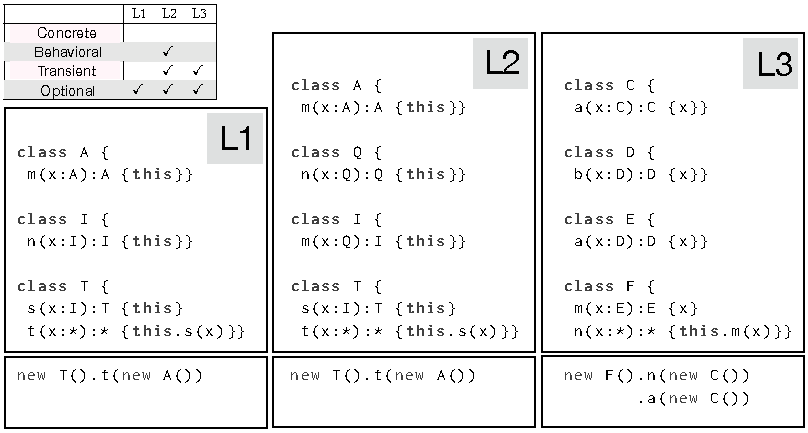
\includegraphics[width=.95\columnwidth]{../figures/litm}
	\caption{Gradual typing litmus test.}\label{litmus}
\end{figure}

{\bf Optional.~} An optional type system, which simply erases all of the
type annotations at runtime, will run all without error.

{\bf Concrete.~} The guarantee provided by the concrete semantics is that
only statically checked values can be of a type, implying that untyped
values can never be passed in placed of a typed one. This strong requirement
causes the concrete semantics to reject all three programs. {\bf L1} fails
as it attempts to pass an \A instance in place of an instance of \xt I,
which are incompatible.  {\bf L2} also fails despite \A and \xt I's
method now being of the same name, the types are statically incompatible due
to \xt Q not being a static super type of \A. {\bf L3} fails as it tries to
pass a \C as an \xt E, in the call to \m inside of \xt N in \xt F,
impossible under the concrete semantics as \C is not a subtype of \xt E.

{\bf Behavioral.~} In contrast to the concrete semantics, the behavioral
semantics does allow untyped values to be passed under a type if they are
structurally compatible, but dynamically ensures that the untyped values to
respect the type. Like the concrete semantics, {\bf L1} is rejected as \A's
method, \m, could never be used as \xt I's \xt n. {\bf L2}, however,
executes without error, as while \A.\xt m does not properly implement \xt
I.\xt n, this is never observed dynamically, and the value is therefore
observationally of the ascribed type. {\bf L3} is rejected by the behavioral
semantics, as when the top-level expression calls \xt a on a \xt C that has
been cast to an \xt E, the check that the value (another instance of \xt C)
is structurally compatible with the required type (\xt D), fails.

{\bf Transient.~} The transient semantics further weakens the guarantee,
retaining the structural checks at casts of the behavioral semantics, but
only checks adherence to the locally ascribed type, rather than every
potentially applicable type. Transient fails {\bf L1}, for the same reason
as the other two type systems, and passes {\bf L2}, for the same reason as
the behavioral semantics, as a result, but differs in {\bf L3}. {\bf L3}
failed under the behavioral semantics because the return value of \xt n
carried the type applied by \xt m with it, forcing the \xt C instance to act
like an \xt E.  However, the transient semantics does not check this,
letting the invocation to \xt a succeed.


%%%%%%%%%%%%%%%%%%%%%%%%%%%%%%%%%%%%%%%%%%%%%%%%%%%%%%%%%%%%%%%%%%%%%%%
\section{Translating Gradual Type Systems}

%\epigraph{\small\it ``Was ist mit mir geschehen? dachte er. Es war kein Traum''}\vspace{-2mm}

\noindent
We are now ready to translate the four gradual type semantics into \kafka.
For each semantics, compilation into \kafka is realized by a translation
function that maps well-typed source programs into well-typed \kafka terms,
respecting a uniform mapping of source types to \kafka types.  The
compilation makes explicit which type casts (and, in turn, \emph{dynamic
  type-checks}) are implicitly inserted and performed by the runtime of each
semantics, highlighting the similarities and differences between them.  Our
source languages, those being translated to \kafka, have no explicit casts,
instead silently coercing types at typed-untyped boundaries, allowing code
like the following:

\begin{tabbing}
\hspace{1cm}\K\HS \Call{\New\C{}}\m{\New\D{}} \HS\HS\HS\WHERE\HS
  \K\HS =\HS \= \class\= \C \{\\
       \> \HS \Mdef\m\x\any\C{\HS\x\HS}\\
       \> \}  \\
       \>\class \D \{ \}
\end{tabbing}         

\noindent The method \m takes an argument of type \any and returns the same
value under type \C. Without a cast, this operation is patently unsafe, as
if \m is passed a \D, the return type of \m will be wrong. However, our
source language allows this, instead deferring to the translation to provide
a safety guarantee.  To avoid unnecessary clutter, we present a common
syntax, reported in \figref{f:sourcesyntax}, for the source language. This
defines a simple object calculus similar to \kafka, but without method
overloading and, most importantly, cast operations. Lastly, we give a
source-level type system for each semantics (notated $\vdash_{\!s}$), which
are largely identical. To simplify the presentation, we will elide rules
identical to those in \kafka, and present only the altered rules.

%TODO: Like types are removed from the figure
\begin{figure}[!h]\hrulefill
	
	\begin{tabular}{ll}
		\begin{minipage}{6cm}\begin{tabular}{@{}l@{~}l@{}l@{}l@{}l@{}l@{}l@{}l}
				\e\hspace{.1cm} ::= & \hspace{.2cm} \x        
				&\B \this         
				&\B \FRead\f \\    
				&
				&\B \FWrite\f\e
				&\B \Call\e\m\e \\
				& 
				&\B \that      
				&\B \New\C{\e[1]..}  
		\end{tabular}\end{minipage}&
		\begin{minipage}{5cm}\begin{tabular}{l@{~}l@{}l@{}l}
				~ \k &::= \Class \C {\fd[1]..}{\md[1]..} \\
				~ \t&::= ~ \any  \B   \C  \\ 
				\md &::= \Mdef\m\x\t\t\e \\
				~\fd&::= ~ \Fdef\f\t \\ 
		\end{tabular}\end{minipage} 
	\end{tabular}
	\vspace{2mm} 

\hrulefill

        \caption{Common source language.}\label{f:sourcesyntax}
\end{figure}



\begin{figure}[!h]
  
  \hrulefill  \footnotesize

  \vspace{-5mm}
  
  \hspace{-.5cm}\begin{mathpar}
          \Rule{STG-VAR}{
            ~\\\\  ~\\\\ ~\\\\
            \HasType \Env\x\t
          }{
            \EnvTypeS \Env\K\x\t
          }

          \Rule{STG-GET}{ ~\\\\ ~\\\\
            \HasType \Env\this\C \\\\
            \Fdef\f\t \in \App\K\C
          }{
            \EnvTypeS \Env\K{\FRead\f}\t
          }    

          \Rule{STG-SET}{
            \HasType \Env\this\C \\\\
            {\Fdef\f\t \in \App\K\C} \\\\
            \EnvTypeS \Env\K\e\tp \\\\
            \ConvertE\K{s}\tp\t
          }{
            \EnvTypeS \Env\K{\FWrite\f\e}\t
          }    

          \Rule[width=15em]{STG-CALL}{
            ~\\\\ ~\\\\
            \EnvTypeS \Env\K\e\any \\\\
            \EnvTypeS \Env\K\ep\t 
          }{
            \EnvTypeS \Env\K{\Call\e\m\ep}{\any}
          }    

          \Rule[width=15em]{STG-CALL}{
            \EnvTypeS \Env\K\e\C \\\\
            \EnvTypeS \Env\K\ep\t \\\\
            \Mtype \m{\t[1]}{\t[2]}\in \App\K\C  \\\\
            \ConvertE\K{s}\t{\t[1]}
          }{
            \EnvTypeS \Env\K{\Call\e\m\ep}{\t[2]}
          }    

          \Rule{STG-NEW}{~\\\\
            \Ftype{\f[1]}{\t[1]}.. \in \App\K\C \\\\
            \EnvTypeS \Env\K{\e[1]}{\tp[1]}..\\\\
            \ConvertE\K{s}{\tp[1]}{\t[1]}..
          }{
            \EnvTypeS \Env\K{\New\C{\e[1]..}}\C
          }
          \end{mathpar}
  
  \vspace{2mm}
  
  \hrulefill
  \caption{Source language type system.}\label{fig:slts}
\end{figure}

The type system for the surface languages is straightforward, allowing
implicit mixing of static and dynamically typed terms, and is shared between
all of the gradual type systems, shown in figure~\ref{fig:slts}.  The
difference between a gradually typed language and a language with the \any
type is the ability to implicitly down-cast from \any to some known type
\t. The mechanisms which make this operation safe are what differentiate
each gradual typing semantics.  The naive typing rules would not allow an
implicit downcast from \any to a non-\any type, as it is not safe. However,
to make our surface language a gradually typed one, we need to represent the
ability to make some kinds of unsafe type conversion within our type system.

The $\ConvertE\K{s}{\t}{\tp}$ operator is used to denote that type $\t$ is
convertible to one of type $\tp$, and is used both for traditional
down-casting and for conversions of \any to non-\any types. Our definition
of the type convertibility operator is shown in figure~\ref{fig:tyconvert},
denoting the surface level typing judgment as $\EnvTypeS\Env\K\e\t$, for a
term $\t$ having type $\t$.

\begin{figure}[!h]
  \hrulefill  \small  \vspace{-3mm}
  
  \begin{mathpar}
    \Rule{STGC-SUB}{
      \SSub\cdot\K\t\tp
    }{
      \ConvertE\K{s}\t\tp
    }
    
    \Rule{STGC-TOANY}{~
    }{
      \ConvertE\K{s}\t\any
    }
    
    \Rule{STGC-ANYCONC}{~
    }{
      \ConvertE\K{s}\any\t
    }
  \end{mathpar}
  \vspace{-8mm}
  
  \hrulefill
  \caption{Optional type convertibility.}\label{fig:tyconvert}
\end{figure}

In the source language, it is possible to pass subtypes as arguments and new
field values (\RuleRef{STGC-SUB}), as in the \kafka type system.  However,
the source language compatibility relation adds two new cases,
\RuleRef{STGC-TOANY} and \RuleRef{STGC-ANYCONC}, allowing typed values to be
used in place of untyped values and vice versa respectively.  If the source
program type checks correctly, we can proceed with translation to \kafka.
For each of the four semantics, we provide a translation from this common,
gradually typed, source language to the statically-typed \kafka target
language, illustrating how the guarantees provided by each system
influence semantics and performance.


\begin{figure}[!h]
	\begin{tabular}{l@{\HS}l}
	\begin{tabular}{llc@{\hspace{.25cm}}l@{\HS}l@{\HS}l}
		{\scriptsize \bf{Optional}} \\
		\TR[\OTS]\x & = \src \x \\
		\TR[\OTS]\this & = \src{\SubCast\any\this} \\
		\TR[\OTS]{\FRead\f} & = \src{\FRead\f} \\
    \\
	\end{tabular}
	&
	\begin{tabular}{llc@{\hspace{.25cm}}l@{\HS}l@{\HS}l}
		{\scriptsize \bf{Transient}} \\
		\TRG[\TTS]\x\Env & = \src{\SubCast\t\x} & \WHERE & \TypeCk{\K,\Env}\x\t \\
		\TRG[\TTS]\this\Env & = \src\this \\
		\TRG[\TTS]{\FRead\f}\Env & = \src{\SubCast\t{\FRead\f}} & \WHERE & \TypeCk{\K,\Env}\this\C & \\
                             &                              &        & \Ftype\f\t\In\App\K\C \\
	\end{tabular}
	\\ \\
	\begin{tabular}{llc@{\hspace{.25cm}}l@{\HS}l@{\HS}l}		
		{\scriptsize \bf{Behavioral}} \\ 
		\TRG[\BTS]\x\Env &= \src{\x} \\
		\TRG[\BTS]\this\Env &= \src{\this} \\
		\TRG[\BTS]{\FRead\f}\Env  &= \src{\FRead\f} \\
	\end{tabular}
	&
	\begin{tabular}{llc@{\hspace{.25cm}}l@{\HS}l@{\HS}l}		
		{\scriptsize\bf{Concrete}} \\
		\TRG[\CTS]{\x}\Env & = \src \x \\
		\TRG[\CTS]\this\Env &= \src{\this} \\
		\TRG[\CTS]{\FRead\f}\Env        & = \src{\FRead\f}  \\
	\end{tabular}
	\end{tabular}
\caption{Translations for variables and field access.}\label{fig:travar}
\end{figure}

\figref{fig:travar} presents the translation for field access and variables,
with notable exceptions in the transient and optional semantics, these
operations are translated verbatim. The grey background is used to
identify translated \kafka terms. For the optional semantics, we have
eliminated the type of the \this introduction form by casting it to \any. The
optional semantics make no other alterations to these terms, as it has no
guarantee to ensure.  Transient does not guarantee the values passed to
functions or field assignment respect the declared type of those
expressions. Class translation inserts checks for invalid variables upon
method entry, so while the transient translation has to insert casts to
appease the \kafka type system, these casts will never fail. However, fields
are not protected and requires a guard after dereferencing, as values can be
passed through them to violate their types.

\begin{figure}[!h]
	\begin{tabular}{llc@{\hspace{.25cm}}l@{\HS}l@{\HS}l}
		{\scriptsize \bf{Optional}} \\
		\TR[\OTS]{\FWrite\f\e} & = \src{\FWrite\f\ep} & \WHERE & \ep=\TR[\OTS]\e \\
		{\scriptsize \bf{Transient}} \\
		\TRG[\TTS]{\FWrite\f\e}\Env & =  \src{{\FWrite\f\ep}} &\WHERE
		& \TypeCk{\K,\Env}\this\C
		& \Ftype\f\t\In\App\K\C 
		& \ep = \TAG[\TTS]\e\Env\any\\
		{\scriptsize \bf{Behavioral}} \\ 
		\TRG[\BTS]{\FWrite\f\e}\Env &=  \src{\FWrite\f\ep} & \WHERE
		& \TypeCk{\K,\Env}{\this}\C
		& \Ftype\f\t\In\App\K\C 
		& \ep = \TAG[\BTS]\e\Env\t\\
		{\scriptsize \bf{Concrete}} \\
		\TRG[\CTS]{\FWrite\f\e}\Env     & = \src{\FWrite\f\ep} & \WHERE
		& \TypeCk{\K, \Env}\this\C
		& \Ftype\f\t\In\App\K\C
		& \ep = \TAG[\CTS]\e\Env{\t} \\
	\end{tabular}
	
\caption{Translations for field assignment.}\label{fig:trassn}
\end{figure}

Field assignment, presented in \figref{fig:trassn}, illustrates the distinct
continuum provided by each gradual type system. Under the optional
semantics, we simply translate the assignment directly, with no guards or
additional checks. However, in the three remaining semantics, the behavior
differs depending on the strength of the guarantees.  Under the transient
semantics, field assignment is unchecked, deferring type checking to
dereferencing. As a result, we use the analytic translation operator to
translate the argument according to the transient semantics. The type of the
field is erased by targeting the $\star$ type in the translation. Under the
behavioral and concrete semantics, type consistency is guaranteed for the
heap, and the translation for the argument expression is done with the known
type of the field.  One observation from these translations is that the
behavioral and concrete semantics demand the correct type to be returned
from the argument expression, while the transient semantics only needs to be
well-formed. As a consequence, the behavioral and concrete semantics will
raise an error when assigning a value of the wrong type to a field, whereas
the transient semantics will rise an error upon dereference.


\begin{figure}[!h]
	\begin{tabular}{llc@{\hspace{.25cm}}l@{\HS}l@{\HS}l}
		{\scriptsize \bf{Optional}} \\
		\TR[\OTS]{\New\C{\e[1]..}} & = \src{\SubCast\any{\New\C{\ep[1]..}}} &\WHERE 
		& \ep[1] = \TR[\OTS]{\e[1]} .. \\
		{\scriptsize \bf{Transient}} \\
		\TRG[\TTS]{\New\C{\e[1]..}}\Env &=  \src{\New\C{\ep[1]..}} &\WHERE 
		& \Ftype{\f[1]}{\t[1]}\In\App\K\C
		& \ep[1] = \TAG[\TTS]{\e[1]}\Env{\any} ~.. \\
		{\scriptsize \bf{Behavioral}} \\ 
		\TRG[\BTS]{\New\C{\e[1]..}}\Env & = \src{\New\C{\ep[1]..}} &\WHERE 
		& \Ftype{\f[1]}{\t[1]}\In\App\K\C
		& \ep[1] = \TAG[\BTS]{\e[1]}\Env{\t[1]} ~..\\
		{\scriptsize \bf{Concrete}} \\
		\TRG[\CTS]{\New\C{\e[1]..}}\Env &= \src{\New\C{\ep[1]..}}  &\WHERE
		& \Ftype{\f[1]}{\t[1]}\In\App\K\C
		& \ep[1] = \TAG[\CTS]{\e[1]}\Env{\t[1]} ..
	\end{tabular}
	
\caption{Translations for object creation.}\label{fig:tranew}
\end{figure}

\figref{fig:tranew} presents the translation for the object creation
expression.  Apart from the optional semantics, the translation for the
object creation expression is almost identical between the transient,
behavioral, and concrete semantics. The only difference lies in the
recursive translation call for the arguments of the object, whereby each
semantics call their respective translation. The optional semantics require
an additional $\star$ cast easing any typing information from the object.


\begin{figure}[!h]
	\begin{tabular}{llc@{\hspace{.25cm}}l@{\HS}l@{\HS}l}
		{\scriptsize \bf{Transient}} \\
		\TAG[\TTS]\e\Env\t & = \src\ep &\WHERE
		& \TypeCk{\K,\Env}\e\tp
		& \EM{\K\vdash\tp\Sub\t}
		& \ep = \TRG[\TTS]\e\Env \\
		\TAG[\TTS]\e\Env\t &= \src{\SubCast\t\ep} &\WHERE
		& \TypeCk{\K,\Env}\e\tp 
		& \EM{\K\vdash \tp \not \Sub \t}
		& \EM{\ep = \TRG[\TTS]\e\Env} \\
		{\scriptsize \bf{Behavioral}} \\ 
		\TAG[\BTS]\e\Env\t & = \src\ep & \WHERE
		& \TypeCk{\K,\Env}\e\tp
		& \EM{\K\vdash \tp \Sub \t}
		& \ep = \TRG[\BTS]\e\Env\\
		\TAG[\BTS]\e\Env\t & = \src{\BehCast\t\ep} & \WHERE
		& \TypeCk{\K,\Env}\e\tp \HS 
		& \EM{\K\vdash \tp \not \Sub \t}
		& \ep = \TRG[\BTS]\e\Env \\
		{\scriptsize\bf{ Concrete}} \\
		\TAG[\CTS]\e\Env\t &= \src\ep &\WHERE
		& \TypeCk{\K,\Env}\e\tp 
		& \EM{\K\vdash\tp \Sub \t} 
		& \ep = \TRG[\CTS]\e\Env\\
		\TAG[\CTS]\e\Env\t &= \src{\SubCast{\t}\ep} &\WHERE
		& \TypeCk{\K,\Env}\e\tp 
		& \EM{\K\vdash\tp \not\Sub \t}
		& \EM{\ep = \TRG[\CTS]\e\Env} 
	\end{tabular}
	
\caption{Translation for type requirement.}\label{fig:trtype}
\end{figure}

Figure~\ref{fig:trtype} depicts the translation for type requirement. For
this translation, we are given the expression to translate, the environment
to translate against, and the \kafka type of the resulting
expression. Under the optional system, all terms have type \any, rendering a
translation for type requirement redundant.
The transient and concrete semantics use standard dynamic subtyping.
The concrete semantics use classes defined by the programmer, while the
transient semantics alters them during translation. Under the transient
semantics, classes are rewritten with dynamic types in place of static types
in functions and field. This causes the subtyping cast in the context of the
transient class translation to check for the existence of a method of
the required name during dynamic subtyping, rather than required to ensure 
the entire class is type compatible.
The behavioral semantics has the same untyped invocation as transient, but 
provides a stronger guarantee. 
The behavioral semantics guarantee a typed receiver respects the type
it is under, allowing the invocation to call the method under the
expected type and not to verify the return type. An ill-typed return
would be caught by a wrapper before it reaches the caller.


\begin{figure}[!h]
	\begin{tabular}{llc@{\hspace{.25cm}}l@{\HS}l@{\HS}l}
		{\scriptsize \bf{Transient}} \\
		\TRG[\TTS]{\Call{\e[1]}\m{\e[2]}}\Env & = \src{\DynCall{\ep[1]}\m{\ep[2]}} & \WHERE 
		& \TypeCk{\K,\Env}{\e[1]}\any 
		& \ep[1] = \TRG[\TTS]{\e[1]}\Env
		& \ep[2] = \TAG[\TTS]{\e[2]}\Env\any \\ 
		\TRG[\TTS]{\Call{\e[1]}\m{\e[2]}}\Env & = 
		& \WHERE
		& \TypeCk{\K,\Env}{\e[1]}\C  
		& \ep[1] = \TRG[\TTS]{\e[1]}\Env  & \ep[2] = \TAG[\TTS]{\e[2]}\Env{\any} \\
		\multicolumn{2}{l}{\HS\HS\HS\HS\HS\HS\HS\HS\HS
    \src{\SubCast{\D[2]}{\KCall{\ep[1]}\m{\ep[2]}\any\any}}} & & \multicolumn{2}{l}{\Mtype\m{\D[1]}{\D[2]}\In\App\K\C} \\
		{\scriptsize Behavioral} \\ 
		\TRG[\BTS]{\Call{\e[1]}\m{\e[2]}}\Env & = \src{\DynCall{\ep[1]}\m{\ep[2]}} & \WHERE
		&  \TypeCk{\K,\Env}{\e[1]}\any
		&  \ep[1] = \TRG[\BTS]{\e[1]}\Env
		&  \ep[2] = \TAG[\BTS]{\e[2]}\Env\any
		\\
		\TRG[\BTS]{\Call{\e[1]}\m{\e[2]}}\Env & = \src{\KCall{\ep[1]}\m{\ep[2]}{\D[1]}{\D[2]}} & \WHERE 
		& \TypeCk{\K,\Env}{\e[1]}\C 
		& \ep[1] = \TRG[\BTS]{\e[1]}\Env
		& \ep[2] = \TAG[\BTS]{\e[2]}\Env{\D[1]}  \\
		& & &  \multicolumn{2}{l}{\Mtype\m{\D[1]}{\D[2]}\In\App\K\C} \\
		{\scriptsize \bf{Concrete}} \\
		\TRG[\CTS]{\Call{\e[1]}\m{\e[2]}}\Env & = \src{\DynCall{\ep[1]}{\m}{\ep[2]}} & \WHERE &
		\TypeCk{\K,\Env}{\e[1]}\any &  \ep[1]= \TRG[\CTS]{\e[1]}\Env & \ep[2] = \TAG[\CTS]{\e[2]}\Env\any\\
		\TRG[\CTS]{\Call{\e[1]}\m{\e[2]}}\Env & = \src{\KCall{\ep[1]}{\m}{\ep[2]}{\D[1]}{\D[2]}} 
		& \WHERE & \TypeCk{\K,\Env}{\e[1]}\C &  \ep[1] = \TRG[\CTS]{\e[1]}\Env &   \ep[2] = \TAG[\CTS]{\e[2]}\Env{\D[1]} \\ 
		& & & \multicolumn{2}{l}{\Mtype\m{\D[1]}{\D[2]}\In\App\K\C} &  \\
	\end{tabular}
	
\caption{Translations for function invocation.}\label{fig:trafuninv}
\end{figure}


Figure~\ref{fig:trafuninv} depicts the translation of function invocation
for the four semantics. For the optional semantics, we do not know if the
function exists over the object. The translation compensate by having
untyped call operator for every function invocation.  Each semantics has to
make a distinction between safe typed calls and unsafe untyped calls. As a
result, a condition is placed over the type of the receiver, using a sound
call if it is typed, and an dynamic invocation if not.  The transient
semantics is almost identically to the optional semantics for function
invocation on untyped expressions.  A dynamic invocation is generated with a
generated argument and \any as the return type, an expression similar to
those found in Typescript.  In case of sound expressions, the transient
semantics will guarantees the existence, but not the types, of methods. In
conjunction with class translation, which ensures an untyped method will
exist for every typed method, the transient semantics insert a
statically-typed call to the \any-typed invocation site. However, to be
compatible with the dynamic call, the argument still needs to be cast to
\any and the return type needs to be checked against the expected type.
In the concrete semantics any method can be called statically and
dynamically, by generating a dynamic version of all source level methods.
Class translation relies on overloading to provide the two versions of each
method: one with concrete receiver and the other with optionally typed
object.  More precisely, given a concrete method \(\md\) with type \(\t[1]
\to \t[2]\), the concrete translation first generates a method \(\mdp\) with
type \(\kty{\t[1]} \to \kty{\t[2]}\) (protecting the the return value with
appropriate cast to \kty{\t[2]} if necessary).  The concrete translation
also generates a second method \mdpp that wraps \mdp to allow a safe
invocation with type \(\any \to \any\).  Finally, every field \f:\t is
mapped to the corresponding field \f:\kty\t.

%\vspace{-2cm}
\medskip
\begin{figure}[!h]  
  \begin{tabular}{llc@{\hspace{.25cm}}l}    
        
    {\scriptsize \bf{Optional}} \\    
    \TR[\OTS]{\Class\C{\fd[1]..}{\md[1].. }} & =  \src{\Class \C {\fdp[1]..}{\mdp[1].. } } \\     
    & \WHERE \HS\HS\HS \fdp[1] = \src{\Ftype\f\any}..\HS\HS \fd[1] = \Ftype\f\t .. \\     
    & \HS\HS\HS\HS\HS\HS\HS\HS\HS  \mdp[1] = \src{\Mdef\m\x\any\any\ep}..\\   
    & \HS\HS\HS\HS\HS\HS\HS\HS\HS \md[1] = \Mdef\m\x{\t[1]}{\t[2]}\e \\   
    & \HS\HS\HS\HS\HS\HS\HS\HS\HS  \ep = \TR[\OTS]{\e} \\   
        
    {\scriptsize \bf{Transient}} \\   
    \TR[\TTS]{\Class\C{\fd[1]..}{\md[1].. }} & =  \src{\Class \C {\fdp[1]..}{\mdp[1].. } } \\   
    & \WHERE \HS\HS\HS \fdp[1] = \src{\Ftype\f\any} .. \HS    
    \fd[1] = \Ftype\f\t ..\HS\HS \\   
    & \HS\HS\HS\HS\HS\HS\HS\HS\HS \mdp[1] = \src{\Mdef\m\x\any\any{\SubCast\t\x ~; ~\ep[1]}} .. \\    
    & \HS\HS\HS\HS\HS\HS\HS\HS\HS \md[1] = \Mdef\m\x\t\tp\e .. \\   
    & \HS\HS\HS\HS\HS\HS\HS\HS\HS \ep[1] = \TAG[\TTS]\e{\x:\t\,\this:\C}\any~ .. \\        
        
    {\scriptsize \bf{Behavioral}} \\    
    \TR[\BTS]{\Class\C{\fd[1]..}{\md[1].. }} & =  \src{\Class \C {\fd[1]..}{\mdp[1].. } } \\    
    & \WHERE \HS\HS\HS \mdp[1] = \src{\Mdef\m\x\t\tp{\ep[1]}} ..\HS\HS \\   
    & \HS\HS\HS\HS\HS\HS\HS\HS\HS \md[1] = \Mdef\m\x\t\tp{\e[1]} ..\HS\HS \\    
    & \HS\HS\HS\HS\HS\HS\HS\HS\HS \ep[1] = \TRG[\BTS]{\e[1]}{\x:\t\,\this:\C} \\    
        
    {\scriptsize \bf{Concrete}} \\    
    \TR[\CTS]{\Class\C{\fd[1]..}{\md[1].. }} & = \src{ \Class \C{ \fd[1]..}{\mdp[1].. \mdpp[1]..}} \\   
    & \WHERE \HS\HS\HS {\mdp[1]} = \src{\Mdef\m\x{{\t[1]}}{{\t[2]}}{\ep}} .. \\    
    & \HS\HS\HS\HS\HS\HS\HS\HS\HS \md[1] = \Mdef\m\x{\t[1]}{\t[2]}\e .. \\   
    & \HS\HS\HS\HS\HS\HS\HS\HS\HS \ep = \TAG[\CTS]{\e}{\this:\C\,\x:\t[1]}{\t[2]}~  ..\\            
    & \HS\HS\HS\HS\HS\HS\HS\HS\HS {\mdpp[1]} = \src{\Mdef\m\x\any\any{\SubCast\any{\KCall\this\m{\SubCast{{\t[1]}}\x}{\t[1]}{\t[2]}}}} \\     
    & \HS\HS\HS\HS\HS\HS\HS\HS\HS \HS\HS\HS\HS\HS\HS\HS\HS\HS\HS\HS \textbf{\IF} {\t[1]} $\neq$ \any \\    
    & \HS\HS\HS\HS\HS\HS\HS\HS\HS \HS\HS\HS\HS\HS\HS \src{empty} \\     
    & \HS\HS\HS\HS\HS\HS\HS\HS\HS \HS\HS\HS\HS\HS\HS\HS\HS\HS\HS\HS {\bf otherwise}  ..   
  \end{tabular}   
      
 \caption{Translations for class.}     \label{fig:traclass}    
\end{figure}    
\medskip


\figref{fig:traclass} presents the class translation for the four gradual
typing semantics, a key part of their functionality. All need to guard
against untyped code calling typed receivers through the dynamic invocation,
which each handles differently. The optional semantics deals with the
problem by eliminating all typed receivers, but the other systems need to
check argument and return types.  The transient semantics heavily relies
upon class translation to achieve the desired semantics, especially with
relation to how it handles casts. Under the transient semantics, all types
are removed from the method signatures and argument types are instead
checked by the method body itself and return types by the caller. Now, with
no typed methods, structural subtyping becomes equivalent to checking that
all the required method names hold and no more, the cast semantics needed by
the transient semantics.  The behavioral semantics protects typed methods
from untyped callers by means of the generated untyped wrappers, and, as a
result, needs no explicit support for such from its translation.  The most
complex class translation is that of the concrete semantics, which needs to
support both typed and untyped callers calling the same class. Here, it uses
\kafka's type-based overloading to define a special untyped receiver method,
one that is generated if the original method was typed. This receiver method
is then responsible for guarding the typed version of the function.


\begin{figure}[!h]
  \begin{tabular}{l}
    {\scriptsize\bf{Source}} \\
\(
\begin{array}{l@{\,}l}
\Class{\xt F}{}{&\Mdef\m\x{\xt E}{\xt E}\x \\
                &\Mdef\n\x\any\any{\Call\this\m\x}} \\
\end{array}
\) \\
    {\scriptsize\bf{Optional}} \\ 
\(
\begin{array}{l@{\,}l}
\Class{\xt F}{}{&\Mdef\m\x{\any}{\any}\x \\
                &\Mdef\n\x\any\any{\DynCall\this\m\x}} \\
\end{array}
\) \\
    {\scriptsize\bf{Transient}} \\
\(
\begin{array}{l@{\,}l}
\Class{\xt F}{}{&\Mdef\m\x\any\any{\SubCast{\xt E}{\x}; ~ \SubCast{\any}{\x} } \\
                &\Mdef\n\x\any\any{\SubCast{\any}{\x}\sspce 
                \SubCast{\any}{\SubCast{\xt E}{\KCall\this\m{\SubCast\any{\SubCast\any\x}}\any\any}}}} \\
\end{array}
\)\\
    {\scriptsize\bf{Behavioral}} \\
\(
\begin{array}{l@{\,}l}
\Class{\xt F}{}{&\Mdef\m\x{\xt E}{\xt E}\x \\
                &\Mdef\n\x\any\any{\BehCast\any{\KCall\this\m{\BehCast{\xt E}\x}{\xt E}{\xt E}}}} \\
\end{array}
\) \\
    {\scriptsize\bf{Concrete}} \\
\(
\begin{array}{l@{\,}l}
\Class{\xt F}{}{&\Mdef\m\x{\xt E}{\xt E}\x \\
                &\Mdef\n\x\any\any{\SubCast\any{\KCall\this\m{\SubCast{\xt E}\x}{\xt E}{\xt E}}}} \\
\end{array}
\) \\
  \end{tabular}
  
 \caption{Litmus Test 3 Class Translation.} \label{fig:l3trans}
\end{figure}

\figref{fig:l3trans} presents an example of how our translation drives the
semantics.  We will translate class {\xt F}'s definition using each of the
four translations, clearly indicating where the behavior of each program.
Translation under the optional semantics is extremely simple, all types are
erased and all invocations are dynamic. However, the translations become
much more complicated when we introduce guarantees.  The first, but weakest,
gradual type semantics is the transient semantics. Under the transient
semantics, all types are erased from the class.  Argument and return types
are not guaranteed. The transient guarantees only require methods to exist
on a type. A statically typed invocation can be made to an untyped method \m
with only untyped arguments and the return type casted as an \any.  The
weakness of the guarantee provided by the transient semantics means the
return type of a method is not guaranteed and the argument types cannot be
trusted. The behavioral semantics recover these properties by using the
behavioral cast operator. The behavioral semantics inserts wrappers over
methods to ensure safety for declared argument and return types.  However,
there is a cost associated with the behavioral cast, as it is complex and
expensive.  The concrete semantics is similar to the behavioral semantics in
using the typed version of \m, and with similarly semantics to the transient
semantics. Whereby only the values statically checked are allowed to pass
through cast boundary.  In \figref{fig:l3etrans} we present the translation
of a simply class {\xt E}. This example aims to illustrate the difference in
guarantee provided by the difference semantics.

\begin{figure}[!h]
  \begin{tabular}{rl}
  \multicolumn{2}{c}{
  \begin{tabular}{l}
    {\scriptsize\bf{Source}} \\
\(
\begin{array}{l@{\,}l}
\Class{\xt E}{}{&\Mdef\m\x{\xt D}{\xt D}\x } \\
\end{array}
\) 
\end{tabular}}
\\
  \begin{tabular}{l}
    {\scriptsize\bf{Optional}} \\ 
\(
\begin{array}{l@{\,}l}
\Class{\xt E}{}{&\Mdef\m\x{\any}{\any}\x } \\
\end{array}
\) 
\end{tabular}&
  \begin{tabular}{l}
    {\scriptsize\bf{Transient}} \\
\(
\begin{array}{l@{\,}l}
\Class{\xt E}{}{&\Mdef\m\x\any\any{\SubCast{\xt E}\x ; ~ \SubCast{\any}{\x}}} \\
\end{array}
\)
\end{tabular}\\
  \begin{tabular}{l}
    {\scriptsize\bf{Behavioral}} \\
\(
\begin{array}{l@{\,}l}
\Class{\xt E}{}{&\Mdef\m\x{\xt E}{\xt E}\x} \\
\end{array}
\) 
\end{tabular} &
  \begin{tabular}{l}
    {\scriptsize\bf{Concrete}} \\
\(
\begin{array}{l@{\,}l}
\Class{\xt E}{}{&\Mdef\m\x{\xt E}{\xt E}\x} \\
\end{array}
\) 
\end{tabular}\\
  \end{tabular}
  
 \caption{Litmus Test 3 Translation for {\xt E}.}  \label{fig:l3etrans}
\end{figure}

For the transient semantics, when \x is cast to {\xt E}, all of the types on
{\xt E} are erased by the transient class translation. Casting to {\xt E} is
tantamount to asking for the existence of the method \m. In contrast, the
concrete semantics retained the types of \m. A concrete translation that
checks if a class is a subtype of {\xt E} is equivalent to checking if a
method \m that takes and returns an {\xt E} exists.  While the concrete
semantics provide a stronger type guarantee, it comes at the cost of the
ability to migrate between untyped and typed code. Suppose that both the
optional and concrete versions of {\xt E} existed, under different a name
{\xt F}. In that system, only the concrete version of {\xt E} could be used
with the concrete version of {\xt F}. Despite implementing the same
behavior, the optional version of {\xt E} would not be able to be used with
the concrete version of {\xt F}, as statically it does not know \m would
take and return an {\xt E}.  The behavioral semantics is able to use the
same representation for {\xt E} as the concrete semantics. The behavioral
cast allows the behavioral semantics to use an optional typed {\xt E}. In
effect, if an optional typed {\xt E} were passed where a behavioral typed
{\xt E} was expected, then a wrapper, implementing the fully typed {\xt E},
would be generated on top of the untyped, optional typed {\xt E}, ensuring
type safety.

\section{Conclusion}\label{litm}

This paper has introduced \kafka, a framework for comparing the design of
gradual type systems for object-oriented languages. Our approach is to
provide translations from different source language into \kafka. These
translations highlight the different runtime enforcement strategies deployed
by the languages under study. The differences between gradual type systems
are made explicit with a litmus test that demonstrates observable
differences between type systems. 

The key features needed in \kafka are two casts, one structural and one
behavioral, and the ability to extend the class table at runtime.  \kafka
was also carefully engineered to support transparent wrappers.  We provide a
mechanized proof of soundness for \kafka that includes runtime class
generation.  We also demonstrate that \kafka can be straightforwardly
implemented on top of a stock virtual machine.

Going forward there are several issues we wish to investigate further.  We
do not envision supporting nominal subtyping within \kafka will pose
problems, it would only take adding a nominal cast and changing the
definition of classes. Then nominal and structural could coexist. A more
challenging question is how to handle the intricate semantics of Monotonic
Python. For these we would need a somewhat more powerful cast operation.
Rather than building each new cast into the calculus itself, it would be
interesting to axiomatize the correctness requirements for a cast and let
users define their own cast semantics.

Another open question for gradual type system designers is performance of
the resulting implementation.  Performance is one of the major obstacles
obstructing gradual typing from being incorporated into mainstream
languages. To illustrate the impact of performance over the gradual typing
semantics, we will discuss an overview of the impact on performance for each
gradual typing semantics.  Under the optional semantics, types are removed
entirely by translation, with the program effectively becoming untyped. As a
result, the performance of the optional semantics will be identical to that
of a wholly untyped program.  The transient semantics checks types at uses
(e.g. on function return and entry), the act of adding types to a program
introduces more casts and will slow the program down. Additionally, the
transient semantics's checks are needed in fully typed code, providing a
strict performance detriment without additional optimizations.  In contrast,
the behavioral semantics does entirely avoid having to insert casts into
fully-typed code, because its soundness guarantee extends to variables being
of their declared types. The cost it pays for this guarantee, however, is
that the declared types are enforced by heavyweight wrappers, inserted at
many places throughout the program, a problem noticed by real
implementations.  Lastly, the concrete semantics is able to achieve a
guarantee similar to that of the behavioral semantics, but without the
overhead of having to add wrappers, enabled by the strong static guarantee
checked for by the cast operator.

\bibliographystyle{plainurl}% the recommended bibstyle
\bibliography{../../bib/jv,../../bib/all}

\newpage
\appendix
%%%%%%%%%%%%%%%%%%%%%%%%%%%%%%%%%%%%%%%%%%%%%%%%%%%%%%%%%%%%%%%%%%%%%%%%%%%%%
\section{Type system for \kafka}%%%%%%%%%%%%%%%%%%%%%%%%%%%%%%%%%%%%
%%%%%%%%%%%%%%%%%%%%%%%%%%%%%%%%%%%%%%%%%%%%%%%%%%%%%%%%%%%%%%%%%%%%%%%%%%%%%%
\label{appendix:kafka}
\subsection{Well-formedness}

The well-formedness judgments for \kafka are defined for programs, classes, methods, fields, and types.

%\vspace{1cm}

\begin{figure}[!h]
	\footnotesize
\begin{minipage}{\textwidth}\begin{tabular}{ll}  
\begin{minipage}{6cm}\begin{mathpar}  
\opdef{~\WFq{\K~\e~\s}}{\text{Well-formed program}}
\vspace{-3mm}
\IRule{WP}{
  \EnvType\emptyset\s\K\e\t \\\\
  \WFtype\K\s \\\\
  \k \in \K \implies \WF{}\cdot\K\k
}{
  \WFq{\K~\e~\s}
}
\end{mathpar}\end{minipage}& \begin{minipage}{5.5cm}\begin{mathpar} 

\opdef{\WF{}\s\K {\Class\C{\fd[1]..}{\md[1]..}}}{\text{Well-formed class}}
\vspace{-2.5mm}
\IRule{WC}{
 \WF {}{}\K {\fd[1]..} \\\\
 \WF {\this:\C~}\s\K {\md[1]..} \\\\
  \cload{\md[1]..~\fd[1]..}
}{
 \WF {}\s\K {\Class \C {\fd[1]..}{\md[1]..}}
}
\end{mathpar}\end{minipage}\end{tabular}\end{minipage}\end{figure}

% \vspace{-1cm}

% The \xt{nodups} function states that there are no overloaded 
% field or method names within the given field and method definitions. \\

\footnotesize
\opdef{~\WF \Env\s\K \md}{Well-formed methods}
\vspace{-1mm}
\begin{mathpar}
\IRule[width=18em]{WT1}{
 \Envp = \Env{~\Ftype\x\any} \\
 \EnvType \Envp\s\K\e\any\\
 \WFtype\K\any \\
}{
 \WF \Env\s\K {\Mdef\m\x\any\any\e}
}

% \IRule[width=18em]{WT2}{
\IRule{WT2}{
 \Envp = \Env{~\Ftype\x\C}\\ 
 \EnvType \Envp\s\K\e\Cp\\
 \WFtype\K\C \\
 \WFtype\K\Cp \\
}{
 \WF \Env\s\K {\Mdef\m\x\C\Cp\e}
}
\end{mathpar}

\begin{figure}[!h]
	\footnotesize
\begin{minipage}{\textwidth}\begin{tabular}{ll}  
\begin{minipage}[t]{7cm}\begin{mathpar}  
\opdef{~\WFtype \K {\fd}}{\text{Well-formed fields}}
% \vspace{-3mm}
\IRule{WF}{
%  ~\\\\
 \WFtype\K\t 
}{
 \WFtype\K{\Fdef\f\t}
}
\end{mathpar}\end{minipage}& \begin{minipage}[t]{5cm}\begin{mathpar} 
 
\opdef{~\WFtype\K\t}{\text{Well-formed types}}
% \vspace{-3mm}
\IRule{WA}{
  ~\\\\
}{
 \WFtype\K\any
}

\IRule{WC}{
 ~\\\\
 \C \in \K
}{
 \WFtype\K\C
}
\end{mathpar}\end{minipage}\end{tabular}\end{minipage}\end{figure}
\vspace{-0.8cm}
\footnotesize
\opdef{~\WFtype\K\s}{\text{Well-formed heaps}}
\vspace{-3mm}
\begin{mathpar} 
\IRule{WH}{
\Bind\ap{\obj\C{\a[1] ..}}~\in~\s \implies \\\\
\Class\C{\fd[1]..}{\md[1]..}\in\K ~~~\wedge~~~  
\EnvType\cdot\s\K{\a[1]}{\t[1]} ~..
}{
 \WFtype\K\s
}
\end{mathpar}

\subsection{Expression typing}

The expression typing judgments for \kafka includes in ascending order as listed in the formalism:
variable, untyped address, subsumption, field assignment, field read, static method invocation, dynamic method invocation, object creation,
subtype cast, typed address.


\opdef{\EnvType\Env\s\K\e\t}{\e has type \t in environment \Env against heap \s and class table \K}
%\vspace{-2mm}
\begin{mathpar}
\IRule{KT-VAR}{
   ~\\\\
   ~\\\\
   \HasType \Env\x\t
 }{
   \EnvType \Env\s\K\x\t
}

\IRule{KT-SUB}{
  ~\\\\
  \EnvType \Env\s\K\e\tp \\\\
 \StrSub \cdot\K \tp \t
 }{
  \EnvType \Env\s\K\e\t 
}   

\IRule{KT-READ}{
  ~\\\\
  \HasType\Env\this\C \\\\
  \Fdef\f\t \in \App\K\C
}{
  \EnvType \Env\s\K{\FRead\f}\t
}  

\IRule{KT-REFREAD}{
  \s(\a) = \C\{..\} \\\\
  \Fdef\f\t \in \App\K\C
}{
  \EnvType \Env\s\K{\FReadR\a\f}\t
}  

\IRule{KT-WRITE}{
  \HasType\Env\this\C \\\\
  \Fdef\f\t \in \App\K\C \\\\
  \EnvType \Env\s\K\e\t
}{
  \EnvType \Env\s\K{\FWrite\f\e}\t
}    

\IRule[width=12em]{KT-REFWRITE}{
  \s(\a) = \C\{..\} \\\\
  \Fdef\f\t \in \App\K\C \\\\
  \EnvType \Env\s\K\e\t
}{
  \EnvType \Env\s\K{\FWriteR\a\f\e}\t
}  

\IRule[width=16em]{KT-CALL}{
  \EnvType \Env\s\K\e\C \\\\
  \EnvType \Env\s\K\ep\t \\\
  \Mtype\m\t\tp \in \App\K\C 
}{
  \EnvType \Env\s\K{\KCall\e\m\ep\t\tp}\tp
}    

\IRule{KT-DYNCALL}{
  ~\\\\
  \EnvType \Env\s\K\e\any \\\\
  \EnvType \Env\s\K\ep\any
}{
  \EnvType \Env\s\K{\DynCall\e\m\ep}\any
}    

\IRule[width=20em]{KT-NEW}{
  ~\\\\
  \EnvType \Env\s\K{\e[1]}{\t[1]}..\\\\
  \Class \C {\Fdef{\f[1]}{\t[1]}..}{\md[1]..} \in \K
}{
  \EnvType\Env\s\K{\New\C{\e[1]..}}\C
}

\IRule{KT-SUBCAST}{
  \EnvType \Env\s\K\e\tp
}{
  \EnvType \Env\s\K{\SubCast\t\e}\t
}

\IRule{KT-BEHCAST}{
  \EnvType \Env\s\K\e\tp
}{
  \EnvType \Env\s\K{\BehCast\t\e}\t
}

\IRule{KT-REFTYPE}{
  \s(\a) = \obj\C{\ap[1]..}
}{
  \EnvType \Env\s\K\a\C
}

\IRule{KT-REFANY}{
 }{
   \EnvType \Env\s\K\a\any
}
\end{mathpar}

\subsection{Dynamic function}

The \xt{dyn} function returns all the methods with $\star$ type for a particular set of 
signatures of method typing.

\begin{mathpar}
\IRule{DYNE}{
}{
  \dyn{\cdot} = \cdot
}

\IRule{DYN}{
 \dyn{\mt[1]..} = \mtp[1].. \\
}{
  \dyn{\Mtype{\m}{\t}{\t} ~\,\mt[1]..} = \Mtype{\m}{\any}{\any}~\,\mtp[1]..
}
\end{mathpar}

\subsection{Signature function}

The \xt{signature} function returns method typing signatures ($\mt$) of method definitions ($\md$).

\begin{mathpar}
\IRule{SGE}{
}{
  \sign{\cdot} = \cdot
}

\IRule{SG}{
  \md = \Mdef\m\x\t\t\e \\
  \sign{\md[1]..} = \mt[1].. \\
}{
  \sign{\md\,\md[1]..} = \Mtype\m\t\t~~\mt[1]..
}
\end{mathpar}

\subsection{Names function}

The \xt{names} function (\names{\fd[1]..}, \names{\md[1]..}, \names{\mt[1]..}) takes either field definitions, method definitions, or 
method typings, and returns the name of the respective fields or methods.

\subsection{Duplicated method names}

The \xt{nodups} function (\cload{\mt[1]..}, \cload{\md[1]..}) takes either
method definitions or method typings, and ensures there are no duplicates.


\section{Source language well-formedness}

\subsection*{Well-formedness for Concrete}

The well-formedness judgments for Concrete is similar to the well-formedness
judgments of \kafka. The turnstile ($\vdash_{\!s}$) of all source language judgment is
characterized with s.

%\begin{figure}[!h]
	\footnotesize
\begin{minipage}{\textwidth}\begin{tabular}{ll}  
\begin{minipage}{6cm}\begin{mathpar}  
\hspace{-1cm}
\opdef{~\WFpW{\e}{\K}}{\text{Well-formed programs}}
\vspace{-3mm}
\IRule{WP}{
  ~\\\\
  \k \in \K \implies \WFW{}\K\k \\
  \EnvTypeW\Env\K\e\t
}{
  \WFpW\e\K
}
\end{mathpar}\end{minipage}& \begin{minipage}{6.0cm}\begin{mathpar}
%\vspace{-6mm}

\opdef{\WFW{}\s\K {\Class\C{\fd[1]..}{\md[1]..}}}{\text{Well-formed classes}}
\vspace{-1mm}
\IRule[width=25em]{WCL}{
 \cload{\fd[1],\md[1]..} \\
 \fd\in\fd[1]..\implies \WFW {}\K \fd \\
 \md\in\md[1]..\implies \WFW {\text{this}:\C~}\K \md 
}{
 \WFW {}\K {\Class \C {\fd[1]..}{\md[1]..}}
}
\end{mathpar}\end{minipage}\end{tabular}\end{minipage}

\vspace{6mm}

\begin{minipage}{\textwidth}\begin{tabular}{l}  
\begin{mathpar}  
\hspace{-7.5cm}                             
\opdef{~\WFW \Env\s\K \md}{\text{Well-formed methods}}

\vspace{-3mm}

\IRule[width=18em]{WT}{
 \EnvTypeW {\Env{~\Ftype\x\C}~}\K\e\D\\
 \WFtypeW\K\C \\
 \WFtypeW\K\D \\
}{
 \WFW \Env\K {\Mdef\m\x\C\D\e}
}

\IRule[width=18em]{WWT}{
 \EnvTypeW {\Env{~\Ftype\x\t}~}\K\e\tp\\
 \WFtypeW\K\t \\
 \WFtypeW\K\tp \\
 \kty\t = \kty\tp = \any
}{
 \WFW \Env\K {\Mdef\m\x\t\tp\e}
}
\end{mathpar}\end{tabular}\end{minipage}

\vspace{4mm}

\begin{minipage}{\textwidth}\begin{tabular}{ll}  
\begin{minipage}{5cm}\begin{mathpar}  
% \hspace{-1cm}
\opdef{~\WFtypeW \K {\Fdef\f\t}}{\text{Well-formed fields}}
\vspace{-3mm}
\IRule{WF}{
 \WFtypeW\K\t 
}{
 \WFtypeW\K{\Fdef\f\t}
}

\end{mathpar}\end{minipage}& \begin{minipage}{6.0cm}\begin{mathpar} 
\hspace{-2cm}
\opdef{~\WFtypeW\K\t}{\text{Well-formed types}}
\vspace{-3mm}

\IRule{WA}{
}{
 \WFtypeW\K\any
}

\IRule{WC}{
 \C \in \K
}{
 \WFtypeW\K\C
}

\IRule{WW}{
 \C \in \K
}{
 \WFtypeW\K{\CW}
}
\end{mathpar}\end{minipage}\end{tabular}\end{minipage}

\clearpage

\subsection*{Well-formedness for Behavioral, Optional, Transient}

The well-formedness judgments for Behavioral, Optional, and Transient is a subset of the well-formedness judgment for \kafka.

\begin{figure}[!h]
% \vspace{-8mm}
\begin{minipage}{\textwidth}\begin{tabular}{ll}  
\begin{minipage}{4cm}\begin{mathpar} 
\opdef{~$\WFpx{\e}{\K}$}{\text{Well-formed programs}}
%\vspace{-2mm}
\IRule{SWF-PROG}{
  \EnvTypex\Env\cdot\K\e\t \\\\
  \k \in \K \implies \WFx{}\cdot\K\k
}{
  \WFpW\e\K
}
\end{mathpar}\end{minipage}& \begin{minipage}{9.0cm}\begin{mathpar} 

\opdef{\WFx{}\s\K {\Class\C{\fd[1]..}{\md[1]..}}}{\text{Well-formed classes}}
%\vspace{-3mm}
\IRule[width=25em]{SWF-CLASS}{
 \cload{\fd[1]..,\md[1]..} \\
 \fd\in\fd[1]..\implies \WFx {}{}\K \fd \\
 \md\in\md[1]..\implies \WFx {\this:\C~}{}\K \md 
}{
 \WFx {}{}\K {\Class \C {\fd[1]..}{\md[1]..}}
}
\end{mathpar}\end{minipage}\end{tabular}\end{minipage}
\end{figure}

\begin{figure}[!h]
\vspace{2mm}
\opdef{~\WFx \Env{}\K \md}{Well-formed methods}
\begin{mathpar}
\hspace{4mm}

\IRule[width=18em]{SWF-TYMETH}{
 \EnvTypex {\Env{~\Ftype\x\C}~}\K\e\D\\
 \WFtypex\K\C \\
 \WFtypex\K\D \\
}{
 \WFx \Env{}\K {\Mdef\m\x\C\D\e}
}

\IRule[width=18em]{SWF-DYMETH}{
 \EnvTypex {\Env{~\Ftype\x\any}~}\K\e\any\\
 \WFtypex\K\any \\
 \WFtypex\K\any
}{
 \WFx \Env{}\K {\Mdef\m\x\any\any\e}
}
\end{mathpar}
\end{figure}

\begin{figure}[!h]
% \vspace{-8mm}
\begin{minipage}{\textwidth}\begin{tabular}{ll}  
\begin{minipage}{4cm}\begin{mathpar} 
\opdef{~\WFtypex \K {\Fdef\f\t}}{\text{Well-formed fields}}
% \vspace{-3mm}
\IRule{SWF-FIELD}{
 \WFtypex\K\t 
}{
 \WFtypex\K{\Fdef\f\t}
}
\end{mathpar}\end{minipage}& \begin{minipage}{10.0cm}\begin{mathpar} 

\hspace{-5cm}

\opdef{~\WFtypex\K\t}{\text{Well-formed types}}
% \vspace{-3mm}
\IRule{SWT-ANY}{
}{
 \WFtypex\K\any
}

\IRule{SWT-TYPE}{
 \C \in \K
}{
 \WFtypex\K\C
} 
\end{mathpar}\end{minipage}\end{tabular}\end{minipage}
\end{figure}

\clearpage

\section{Source semantics type systems and translations}

To avoid unnecessary clutter, we represent the source languages using the
common syntax reported in \figref{f:sourcesyntax2}.  This defines a simple
object calculus similar to \kafka, but without method overloading and, most
importantly, cast operations. Lastly, we also give a source-level type system for 
each language (notated $\vdash_{\!s}$), which are largely identical. To 
simplify the presentation, we will elide the identical rules, instead presenting
only the altered rules.

\begin{figure}[!h]\hrulefill
	\vspace{2mm}  \small
	
	\begin{tabular}{ll}
		\begin{minipage}{6cm}\begin{tabular}{@{}l@{~}l@{}l@{}l@{}l@{}l@{}l@{}l}
				\e\hspace{.1cm} ::= & \hspace{.2cm} \x        
				&\B \this         
				&\B \FRead\f \\    
				&
				&\B \FWrite\f\e
				&\B \Call\e\m\e \\
				& 
				&\B \that      
				&\B \New\C{\e[1]..}  
		\end{tabular}\end{minipage}&
		\begin{minipage}{5cm}\begin{tabular}{l@{~}l@{}l@{}l}
				~ \k &::= \Class \C {\fd[1]..}{\md[1]..} \\
				~ \t&::= ~ \any  \B   \C \\ 
				\md &::= \Mdef\m\x\t\t\e \\
				~\fd&::= ~ \Fdef\f\t \\ 
		\end{tabular}\end{minipage} 
	\end{tabular}
	\vspace{2mm} 
\caption{Common syntax of source languages.}\label{f:sourcesyntax2}
\end{figure}

\subsection{Optional}

Our formalization of TypeScript's type system is in
\figref{convts2}. The type system relies on the \emph{convertibility}
relation, denoted \ConvertE\K{s}\t\tp, which captures precisely the implicit
type conversions allowed by TypeScript.  The convertible relation appears in
\figref{tsts2} and states that a type is convertible to a super type and
that \any is convertible to anything and conversely. 

\begin{figure}[hb]
	
	\hrulefill  \footnotesize
	
	\hspace{-.5cm}\begin{minipage}{\textwidth}\begin{tabular}{llllll}  
			\hspace{.5cm}
			\begin{minipage}{1cm}\begin{mathpar}  
					\Rule{STG-VAR}{
						~\\\\  ~\\\\ ~\\\\
						\HasType \Env\x\t
					}{
						\EnvTypeS \Env\K\x\t
					}
			\end{mathpar}\end{minipage}
			&
			\begin{minipage}{0.5cm}\begin{mathpar}
					\Rule{STG-GET}{ ~\\\\ ~\\\\
						\HasType \Env\this\C \\\\
						\Fdef\f\t \in \App\K\C
					}{
						\EnvTypeS \Env\K{\FRead\f}\t
					}    
				\end{mathpar}
			\end{minipage} & \hspace{-1cm}
			\begin{minipage}{3.2cm}\begin{mathpar}  
					\Rule{STG-SET}{
						\HasType \Env\this\C \\\\
						{\Fdef\f\t \in \App\K\C} \\\\
						\EnvTypeS \Env\K\e\tp \\\\
						\ConvertE\K{s}\tp\t
					}{
						\EnvTypeS \Env\K{\FWrite\f\e}\t
					}    
			\end{mathpar}\end{minipage}& \begin{minipage}{3cm}\begin{mathpar}  
					\Rule[width=15em]{STG-CALL}{
						~\\\\ ~\\\\
						\EnvTypeS \Env\K\e\any \\\\
						\EnvTypeS \Env\K\ep\t 
					}{
						\EnvTypeS \Env\K{\Call\e\m\ep}{\any}
					}    
			\end{mathpar}\end{minipage} \\
			\hspace{.3cm}
			\begin{minipage}{2.8cm}\begin{mathpar}  
					\Rule[width=15em]{STG-CALL}{
						\EnvTypeS \Env\K\e\C \\\\
						\EnvTypeS \Env\K\ep\t \\\\
						\Mtype \m{\t[1]}{\t[2]}\in \App\K\C  \\\\
						\ConvertE\K{s}\t{\t[1]}
					}{
						\EnvTypeS \Env\K{\Call\e\m\ep}{\t[2]}
					}    
			\end{mathpar}\end{minipage} & \hspace{.3cm} \begin{minipage}{3cm}\begin{mathpar}  
					\Rule{STG-NEW}{~\\\\
						\Ftype{\f[1]}{\t[1]}.. \in \App\K\C \\\\
						\EnvTypeS \Env\K{\e[1]}{\tp[1]}..\\\\
						\ConvertE\K{s}{\tp[1]}{\t[1]}..
					}{
						\EnvTypeS \Env\K{\New\C{\e[1]..}}\C
					}
	\end{mathpar}\end{minipage}\end{tabular}\end{minipage}
	
	\vspace{2mm}
	
	\hrulefill
	\caption{Optional type system.}\label{convts2}
\end{figure}

The TypeScript compiler translates code to JavaScript with all types erased.
Since convertibility allows arbitrary values can be passed whenever a \any
value is expected, method calls may fail because the receiver need not have
the requested method. The designers of TypeScript saw this unsoundness as a
way to ensure that types do not get in the way of running correct programs,
e.g. when importing a new library with type annotations inconsistent with
existing client code; and an insurance for backwards compatibility, as
ignoring types means all browsers can run TypeScript code -- with no
additional overhead.

\begin{figure}[hb]
	\hrulefill  \small  \vspace{-3mm}
	
	\begin{mathpar}
		\Rule{STGC-SUB}{
			\SSub\cdot\K\t\tp
		}{
			\ConvertE\K{s}\t\tp
		}
		
		\Rule{STGC-TOANY}{~
		}{
			\ConvertE\K{s}\t\any
		}
		
		\Rule{STGC-ANYCONC}{~
		}{
			\ConvertE\K{s}\any\tp
		}
	\end{mathpar}
	\vspace{-8mm}
	
	\hrulefill\caption{Optional type convertibility.}\label{tsts2}
\end{figure}


\begin{figure}[hb]	
	\hrulefill
	
	\smallskip
	
	\begin{tabular}{@{}l@{~ ~ ~ ~~~~~~~~~~~~~~~~~~~~~~~~~~~~~~~~~~~~}ll}
		\small
		\begin{minipage}{8cm}  
			\begin{tabbing}
				\TR{\Class \C{\fd[1]..}{\md[1] .. } } = \src{ \Class \C{ \fdp[1]..}{\mdp[1]..}}\\ \HS\HS\HS\HS\HS\HS\HS\HS\HS\HS\HS\HS\HS\HS\HS\HS \WHERE\HS
				\=\fdp[1] = \src{\Ftype\f\any}..\HS\HS\=\fd[1] = \Ftype\f\t .. \HS\HS\=\md[1] = \Mdef\m\x{\t[1]}{\t[2]}\e \\
				\>\mdp[1] = \src{\Mdef\m\x\any\any\ep}..\HS\HS \>\>\ep = \TR{\e}
			\end{tabbing}
			\begin{tabbing}
				\TR{\FRead\f}\HS\HS\HS\HS\= = \src{\FRead\f}
				\\
				\TR{\FWrite\f\e} \> = \src{\FWrite\f\ep} \HS\HS\HS\HS\HS\=\WHERE~\ep=\TR\e
				\\
				\TR\this           \>= \src{\SubCast\any\this}
				\\
				\TR\x \> = \src \x
				\\
				\TR{\Call{\e[1]}\m{\e[2]}} \> = \src{\DynCall{\ep[1]}{\m}{\ep[2]}} \HS\>\WHERE\HS\ep[1] = \TR{ \e[1]} \HS \ep[2] = \TR{\e[2]}
				\\
				\TR{\New\C{\e[1]..}} \> = \src{\SubCast\any{\New\C{\ep[1]..}}} \HS \>\WHERE \HS   \ep[1] = \TR{\e[1]} ..
			\end{tabbing}
		\end{minipage}
	\end{tabular}
	
	\smallskip
	\hrulefill
	\caption{Optional translation.}\label{tst2}
	
\end{figure}

Observe that the optional translations, in \figref{tst2}, does insert some structural casts
to \any, they are needed for the result to be well-typed, but these have no
operational effect (a structural cast to \any always succeed at runtime).
The unsoundness of the optional type system is evidence in the
translation, by discarding the type of the callee and systematically relying
on dynamic method invocation for method calls it clear that optional
programs can get stuck at any point of their execution.

\clearpage

\subsection{Concrete}

The formalization of the Thorn type system is built on top of the rules
presented for TypeScript in \figref{tsts2} and \figref{convts2}. The
definition of subtyping is extended to account for optional types, this 
appears in \figref{subth2}. Optional types are subtypes if the corresponding
concrete types are subtypes. Concrete types are subtypes of optional types,
if the relation holds on concrete types. The convertibility rule must be
extended by one case, as shown in \figref{convth2}, this extra rule states
that an optional type is convertible to a concrete parent type. Type rule
for method calls, shown in \figref{thts2} must be extended to handle
receivers of optional types, they are treated as if they were concrete
types.

\begin{figure}[hb]
	
	\hrulefill  \small
	\vspace{-3mm}
	
	\begin{mathpar}
		\Rule{TSWeak}{
			\SSub \M\K\C\D
		}{
			\SSub \M\K{\dt\C}{\dt\D}
		}
		
		\Rule{TSLow}{
			\SSub \M\K\C\D
		}{
			\SSub \M\K{\C}{\dt\D}
		}
	\end{mathpar}
	
	\hrulefill
	\caption{Concrete subtyping.}\label{subth2}
\end{figure}	

\begin{figure}[hb]	
	\hrulefill  \small
	\vspace{-3mm}
	
	\begin{mathpar}
		\Rule{STHC-OPTCONC}{
			\SSub\cdot\K\C\D
		}{
			\ConvertE\K{th}\CW\D
		}
	\end{mathpar}
	
	\hrulefill
	\caption{Concrete type convertibility.}\label{convth2}
\end{figure}	

\begin{figure}[hb]	
	
	\hrulefill  
	\vspace{0.5mm}
	
	\begin{mathpar}  
		\Rule{STH-CALL}{
			\EnvTypeW \Env\K\e\tp \\  (\tp=\C~~\vee~~\tp=\CW) \\
			\Mtype \m{\t[1]}{\t[2]}\in \App\K\C  \\
			\EnvTypeW \Env\K\ep\tpp  \\
			\ConvertE\K{th}\tpp{\t[1]}
		}{
			\EnvTypeW \Env\K{\Call\e\m\ep}{\t[2]}
		}    
	\end{mathpar}
	
	\hrulefill
	\caption{Concrete type system.}\label{thts2}
\end{figure}	

The translation of Thorn into \kafka is given in~\figref{thtr2}. As with
TypeScript translation proceeds top-down. The differences are that the
translation function for expressions, \TRG{\e}\Env, takes a source-level
typing environment as input. This is used to record the expect type of \this
and arguments \x to methods. Furthermore, the translation can also request
the insertion of casts, this is done with the function \TAG{\e}\Env\t which
translates an expression and ensures that the result is of type \t. The most
interesting case in the translation is the handling of method invocation
\Call\e\m\ep. If the type of \e is a concrete \C, then a statically resolved
invocation of the form \KCall\e\m\ep\t\tp will be emitted. If \e is dynamic
or an optional type, then a dynamically resolved call of the form
\DynCall\e\m\ep is emitted.  The argument of statically resolved method
invocation, as well as constructors and field assignment are all translated
using the auxiliary function as their expected type is known.  This function
translates its argument, checks if its type is a subtype of the expected
type \t, and if not it inserts the appropriate cast.  The cast is performed
in the \kafka type system, and not in the source type system, and must
respect the mapping from Thorn types to \kafka types.  This mapping is
defined by the \kty\t function: \kty\t = \any if \t=\dt\C or \t=\any, \t
otherwise.  Thorn optional and dynamic types are mapped to the \any type,
while concrete types are unchanged.

\begin{figure}[hb]	
	\hrulefill
	\vspace{4mm}	
	\hrulefill
	\medskip
\begin{tabular}{@{}l@{~ ~ ~ ~~~~~~~~~~~~~~~~~~~~~~~~~~~~~~~~~~~~}ll}
	\small
	\begin{minipage}{8cm}  
		\begin{tabbing}
			\TR{\Class \C{\fd[1]..}{\md[1].. }}\= = \src{ \Class \C{ \fdp[1]..}{\mdp[1]..~ \mdpp[1]..}} 
			\HS \WHERE \\ \> {\fdp[1]} = \src{\Ftype\f{\kty\t}} .. \LS\LS\LS \=\fd[1] = \Ftype\f\t ..   \\
			\> {\mdp[1]} = \src{\Mdef\m\x{\kty{\t[1]}}{\kty{\t[2]}}{\ep}} .. \\ \>  \= \md[1] = \Mdef\m\x{\t[1]}{\t[2]}\e ..\HS\HS\= \ep = \TAG{\e}{\HT\this\C\,\HT\x{\t[1]}}{\t[2]} ..\\
			\> {\mdpp[1]} = \src{\Mdef\m\x\any\any{\SubCast\any{\KCall\this\m{\SubCast{\kty{\t[1]}}\x}{\t[1]}{\t[2]}}}} \\
			\>\hspace{1cm}\HS\HS\HS\HS\HS\HS \textbf{\IF} \kty{\t[1]} = \D \textbf{\OR} \kty{\t[2]} = \D\\
			\>\hspace{1cm} empty \HS  {\bf otherwise}  ..                  
		\end{tabbing}
		\begin{tabbing}
			\TRG{\x}\Env\hspace{1.4cm}\= = \src \x
			\\
			\TRG{\FRead\f}\Env        \> = \src{\FRead\f} 
			\\
			\TRG{\FWrite\f\e}\Env     \> = \src{\FWrite\f\ep} \hspace{.5cm}
			\=\WHERE\HS \TypeCk{\K, \Env}\this\C \HS\HS\=  \Ftype\f\t\In\App\K\C \HS\HS\= \ep = \TAG\e\Env{\kty\t}
			\\
			\TRG{\Call{\e[1]}\m{\e[2]}}\Env \>= \src{\DynCall{\ep[1]}{\m}{\ep[2]}} 
			\>\WHERE\HS \TypeCk{\K,\Env}{\e[1]}\t \> \kty\t=\any \>  \ep[1]= \TRG{\e[1]}\Env \= \\ 
			\> \> \HS\HS\HS\HS\HS\HS\HS \ep[2]=\TAG{\e[2]}\Env\any
			\\
			\TRG{\Call{\e[1]}\m{\e[2]}}\Env \>= \src{\KCall{\ep[1]}{\m}{\ep[2]}{\t[2]}{\tp[2]}} 
			\>\WHERE\HS \TypeCk{\K,\Env}{\e[1]}\C \>  \ep[1] = \TRG{\e[1]}\Env \>   \ep[2] = \TAG{\e[2]}\Env{\t[2]} \\ 
			\> \> \HS\HS\HS\HS\HS\HS\HS \Mtype\m{\t[1]}{\tp[1]}\In\App\K\C \>
			\t[2] = \kty{\t[1]} \> \tp[2] = \kty{\tp[1]}
			\\
			\TRG{\New\C{\e[1]..}}\Env\> = \src{\New\C{\ep[1]..}} 
			\>\WHERE\HS \Ftype{\f[1]}{\t[1]}\In\C \> \ep[1] = \TAG{\e[1]}\Env{\t[1]} ..
			\\
			\TAG\e\Env\t\> = \src\ep 
			\>\WHERE\HS  \TypeCk{\K,\Env}\e\tp \> \ep = \TRG\e\Env \\
			\> \> \HS\HS\HS\HS\HS\HS\HS \EM{\K\vdash\kty\tp \Sub \kty\t}
			\\
			\TAG\e\Env\t \>= \src{\SubCast{\kty\t}\ep}
			\>\WHERE\HS   \TypeCk{\K,\Env}\e\tp \> \ep = \TRG\e\Env \\
			\> \> \HS\HS\HS\HS\HS\HS\HS \EM{\K\vdash\kty\tp \not\Sub \kty\t} 
		\end{tabbing}
	\end{minipage}
\end{tabular}
	
	\medskip
	
	\hrulefill
	\caption{Concrete translation.}\label{thtr2}
\end{figure}

\clearpage

\subsection{Behavioral}

The translation for Typed Racket, shown in \figref{trtr2} maps classes to
homonymous classes and types to types of the same name. The \kty{t} function
is the identity.  Calls with a receiver of type \any are translated to
\kafka dynamic calls, and calls with a receiver of some type \C are
translated to statically typed calls. The auxiliary type-directed
translation function \TAG\e\Env\t introduces behavioral casts to \any or \C
appropriately. Thus casts can appear are at typed/untyped boundaries in
assignment, argument of calls or constructors. Because of the strong
guarantee provided by the behavioral cast, the Typed Racket translation is
straightforward. In Typed Racket, every typed value is assumed to behave as
specified, delegating the complexity of checking for consistency with the
type to the wrapper introduced by the behavioral cast.  So the difference
with the TypeScript translation is that typed code is able to use typed
accesses. The difference with Thorn is essentially the presence of wrappers
and the fact that each wrapper application only check the presence of
methods names rather than complete signatures for concrete types.

\begin{figure}[!b]
	
	\hrulefill
	
	\medskip
	
	\small
	\begin{minipage}{12cm}  
		\begin{tabbing}
			\TR{\Class\C{\fd[1]..}{\md[1].. }} =  \src{\Class \C {\fd[1]..}{\mdp[1].. } }\\
			\hspace{4.6cm}\= \WHERE\HS 
			\mdp[1] = \src{\Mdef\m\x\t\tp{\ep[1]}} ..\HS\HS \\
			\>\qquad\HS\HS\HS\HS\md[1] = \Mdef\m\x\t\tp{\e[1]} ..\HS\HS \\
			\>\qquad\HS\HS\HS\HS \ep[1] = \TRG{\e[1]}{\x:\t\,\this:\C}
			\\
			\TRG\x\Env = \src{\x}
			\\
			\TRG{\FRead\f}\Env  = \src{\FRead\f}
			\\
			\TRG{\FWrite\f\e}\Env =  \src{\FWrite\f\ep} 
			\>\WHERE\HS
			\= \TypeCk\K{\this}\C \HS\HS
			\=  \ep = \TAG\e\Env\t \HS\HS
			\= \Ftype\f\t\In\App\K\C
			\\
			\TRG{\Call{\e[1]}\m{\e[2]}}\Env = \src{\DynCall{\ep[1]}\m{\ep[2]}}
			\>\WHERE \> \TypeCk{\K,\Env}{\e[1]}\any \HS
			\> \ep[1] = \TRG{\e[1]}\Env \HS
			\> \ep[2] = \TAG{\e[2]}\Env\any
			\\
			\TRG{\Call{\e[1]}\m{\e[2]}}\Env = \src{\KCall{\ep[1]}\m{\ep[2]}{\D[1]}{\D[2]}}
			\>\WHERE \> \TypeCk{\K,\Env}{\e[1]}\C 
			\> \ep[1] = \TRG{\e[1]}\Env\HS\HS
			\> \ep[2] = \TAG{\e[2]}\Env{\D[1]} \HS\HS \\
			\> \> \=  \Mtype\m{\D[1]}{\D[2]}\In\App\K\C 
			\\
			\TRG{\New\C{\e[1]..}}\Env =  \src{\New\C{\ep[1]..}}
			\>\WHERE \>  \ep[1] = \TAG{\e[1]}\Env{\t[1]} ~..
			\> \HS\HS\HS\HS\HS\HS\HS\HS\HS\HS \Ftype{\f[1]}{\t[1]}\In\App\K\C ~..
			\\
			\TAG\e\Env\t = \src\ep
			\> \WHERE\> \TypeCk{\K,\Env}\e\tp \HS
			\>\HS\HS\HS\HS\HS\HS\HS\HS\HS\HS \EM{\K\vdash \t \Sub \tp}
			\>\ep = \TRG\e\Env
			\\
			\TAG\e\Env\t = \src{\BehCast\t\e}
			\>\WHERE\> \TypeCk{\K,\Env}\e\tp \HS 
			\>\HS\HS\HS\HS\HS\HS\HS\HS\HS\HS  \EM{\K\vdash \t \not \Sub \tp}
			\> \ep = \TRG\e\Env
		\end{tabbing}
	\end{minipage}
	
	\medskip
	
	\hrulefill
	\caption{Behavioral translation.}\label{trtr2}
\end{figure}

\subsection{Transient}

The Transient static type system is based on TypeScript except that the
convertibility rules now builds on an auxiliary \emph{consistency} relation,
defined in~\figref{subtp2} to relate types \t and \tp. The modified
convertibility rule appears in \figref{convtp2}. Consistent subtyping holds
between types with signatures that agree up to \any.  It is worth observing
that the Transient runtime does not use consistent subtyping, instead it
merely validates that all required method names are present.

\begin{figure}[!t]
	\hrulefill
	\vspace{-4mm}
	
	\begin{mathpar}
		\Rule{STTC-SUB}{
			\ConSub\cdot\K\t\tp
		}{
			\ConvertE\K{tr}\t\tp
		}
	\end{mathpar}
	\vspace{-6mm}
	
	\hrulefill
	\caption{Transient convertibility.}\label{convtp2}
\end{figure}	
\begin{figure}[hb]		
	
	\hrulefill
	\small\vspace{-4mm}
	
	\begin{mathpar} 
		\Rule{CSCons}{
			~
		}{
			\ConSub\M\K \any \C
		}
		
		\Rule{CSCons}{
			~
		}{
			\ConSub\M\K \C \any
		}
		
		\Rule{CSCons}{
			~
		}{
			\ConSub\M\K \t \t
		}
		
		\Rule{CSAss}{
			\C \Sub \D \in \M
		}{
			\ConSub \M\K \C\D
		}
		
		\Rule{CSRec}{
			\M' = \M~\C\Sub\D \\\\
			\mt \in \App\K\D \implies 
			\mtp \in \App\K\C ~~~\wedge~~~   \ConSub{\M'}\K\mt{\mtp}
		}{
			\ConSub \M\K \C \D 
		}
		
		\Rule{CSMet}{
			\ConSub \M\K {\t[2]} {\t[1]} \\
			\ConSub \M\K {\tp[1]} {\tp[2]}
		}{
			\ConSub \M\K {\Mtype\m{\t[1]}{\tp[1]}} {\Mtype\m{\t[2]}{\tp[2]}}
		}
	\end{mathpar}
	
	\hrulefill
	\caption{Transient consistent subtyping.}\label{subtp2}
\end{figure}	

\clearpage

\begin{figure}[hb]		
	\hrulefill
	\vspace{1mm}
	
	\begin{tabular}{@{}l@{~ ~ ~}ll}
		\small
		\begin{minipage}{8cm}  
			\begin{tabbing}
				\TR{\Class\C{\fd[1]..}{\md[1].. }} =  \src{\Class \C {\fdp[1]..}{\mdp[1].. } }\\
				\hspace{.5cm}  \WHERE\HS \=
				\fdp[1] = \src{\Ftype\f\any} .. \HS
				\fd[1] = \Ftype\f\t ..\HS\HS
				\mdp[1] = \src{\Mdef\m\x\any\any{\SubCast\t\x ~; ~\ep[1]}} .. \\
				\HS\HS\HS\HS\HS\HS\HS\HS\HS\HS
				\md[1] = \Mdef\m\x\t\tp\e .. 
				\HS\HS
				\ep[1] = \TAG\e{\x:\t\,\this:\C}\tp~ ..
			\end{tabbing}
			\begin{tabbing}
				\TRG\this\Env \hspace{1cm} \= = \src\this
				\\
				\TRG\x\Env \>= \src{\SubCast\t\x} \hspace{1.5cm} \=\WHERE \HS \TypeCk{\K,\Env}\x\t
				\\
				\TRG{\FRead\f}\Env \>= \src{\SubCast\t{\FRead\f}} \>\WHERE\HS  \TypeCk{\K,\Env}\this\C \HS\HS\= \Ftype\f\t\In\App\K\C
				\\
				\TRG{\FWrite\f\e}\Env \>=  \src{\SubCast\t{\FWrite\f\ep}}
				\>\WHERE\HS
				\TypeCk{\K,\Env}\this\C
				\> \Ftype\f\t\In\App\K\C \\
				\> \> \HS\HS\HS\HS\HS\HS\HS  \= \ep = \TAG\e\Env\any
				\\
				\TRG{\Call{\e[1]}\m{\e[2]}}\Env \>= \src{\DynCall{\ep[1]}\m{\ep[2]}}
				\>\WHERE \HS 
				\TypeCk{\K,\Env}{\e[1]}\any 
				\> \HS\HS\HS\HS\HS\HS\HS\HS\HS\HS\HS\HS \ep[1] = \TRG{\e[1]}\Env \\
				\> \> \HS\HS\HS\HS\HS\HS\HS \ep[2] = \TAG{\e[2]}\Env\any
				\\
				\TRG{\Call{\e[1]}\m{\e[2]}}\Env \>= \src{\SubCast\tp{\KCall{\ep[1]}\m{\ep[2]}\any\any}}
				\>\WHERE\HS
				\TypeCk{\K,\Env}{\e[1]}\C
				\> \HS\HS\HS\HS\HS\HS\HS\HS\HS\HS\HS\HS \Mtype\m\t\tp\In\App\K\C\HS \\
				\> \> \HS\HS\HS\HS\HS\HS\HS \ep[1] = \TRG{\e[1]}\Env \HS\HS\HS\HS\=
				\ep[2] = \TAG{\e[2]}\Env\any
				\\
				\TRG{\New\C{\e[1]..}}\Env \>=  \src{\New\C{\ep[1]..}} \>\WHERE\HS
				\Ftype{\f[1]}{\t[1]}\In\App\K\C
				\>\ep[1] = \TAG{\e[1]}\Env{\any} ~..
				\\
				\TAG\e\Env\t \>= \src{\SubCast\t\ep}
				\>\WHERE\HS \TypeCk{\K,\Env}\e\tp 
				\> \EM{\ConSub{}\K\t\tp} \\
				\> \> \HS\HS\HS\HS\HS\HS\HS \EM{\K\vdash\t\not{<:}\tp}  
				\> \EM{\ep = \TRG\e\Env}
				\\
				\TAG\e\Env\t \>= \src\ep \>\WHERE\HS  \TypeCk{\K,\Env}\e\tp
				\>\EM{\K\vdash\t\Sub\tp} \HS \\
				\> \> \HS\HS\HS\HS\HS\HS\HS \ep = \TRG\e\Env
			\end{tabbing}
		\end{minipage}
	\end{tabular}
	
	\medskip
	
	\hrulefill
	
	\caption{Transient translation.}\label{tptr2}
\end{figure}

The Transient translation appears in \figref{tptr2}. Each class is translated
to a homonymous \kafka class, field types are translated to \any, method
types are given the $\any \to \any$ signature. Since argument and return
types are erased, our translation can use structural casts to implement
Transient runtime checks. They degenerate to simple inclusion checks on
method names.  The translation of method invocation makes explicit the
Transient guarantee.  A method call \Call\e\m\ep is translated to
\KCall\e\m\ep\any\any if the type \e is not \any. This translation combined
with the soundness of \kafka entails that the method call will not get
stuck.  Of course of \e is of type \any, the call will be translated to
\DynCall\e\m\ep which can get stuck.  To achieve that guarantee the
translation must insert structural casts at every expression read. Transient
also checks arguments of methods, since the expression may not use the
argument (but Transient checks it anyway) our translation generates method
bodies of the form \SubCast\t\x; \e where \e is the body of the expression
and the semi colon is syntactic sugar for sequencing. Likewise, in order to 
ensure that field assignment will not get stuck, Transient gives all fields 
type \any, then checks the field value on reads based on the static typing.

\clearpage

\section{Litmus tests}

Below we present source code for each of the litmus tests of \figref{litmus}
of section \ref{litmustest}. 

\subsection*{Concrete}

The code for the litmus tests in Thorn. \\ 

\noindent
\textbf{Litmus Test 1}:
\begin{verbatim}
class A() { def m(x:A):A = this; }
class I() { def n(x:I):I = this; }
class T() {
  def s(x:I):T = this;
  def t(x:dyn):dyn = this.s(x);
}
T().t(A());
\end{verbatim}

\noindent
\textbf{Litmus Test 2}:
\begin{verbatim}
class Q() { def n(x: Q): Q = this;}
class A() { def m(x:A): A = this;}
class I() { def m(x:Q):I = this;}
class T() {
   def s(x:I):T = this; 
   def t(x:dyn):dyn = this.s(x);
}
T().t(A());   
\end{verbatim}


\noindent\textbf{Litmus Test 3}:
\begin{verbatim}
class C() { def m(x:C):C = x; }
class D() { def n(x:D):D = x; }
class E() { def m(x:D):D = x; }      
class F() {
   def m(x:E):E = x;
   def n(x:dyn):dyn = this.m(x);
} 
F().n(C()).m(C());
\end{verbatim}

\subsection*{Optional}

The code for the litmus tests in TypeScript. \\

\noindent\textbf{Litmus Test 1}:
\begin{verbatim}
class A { m(x: A): A { return this } }
class I { n(x:I):I { return this } }
class T {
    s(x: I): T { return this }
    t(x: any): any { return this.s(x) }
}
new T().t(new A())
\end{verbatim}

\noindent\textbf{Litmus Test 2}:
\begin{verbatim}
class Q { n(x: Q): Q { return this } }
class A { m(x: A): A { return this } }
class I { m(x:Q):I { return this } }
class T {
    s(x: I): T { return this }
    t(x: any): any { return this.s(x) }
}
new T().t(new A())
\end{verbatim}

\noindent\textbf{Litmus Test 3}:
\begin{verbatim}
class C { m(x: C): C { return x } }
class D { n(x: D): D { return x } }
class E { m(x: D): D { return x } }
class F {
    m(x: E): E { return x }
    n(x: any): any { return this.m(x) }
}
new F().n(new C()).m(new C())
\end{verbatim}

\subsection*{Behavioral}

The code for the litmus tests in Typed Racket. \\

\noindent\textbf{Litmus Test 1}:

\begin{verbatim}
#lang racket
(module u racket
  (define Tp% (class object%
                (super-new)
                (define/public (t x) (send this s x))))
  (provide Tp%))
(module t typed/racket
  (require/typed (submod ".." u) [Tp% (Class [t (-> Any Any)])])
  (define-type A (Instance (Class (m (-> A A)))))
  (define-type I (Instance (Class (n (-> I I)))))
  (define-type T (Instance (Class (s (-> I T)))))
  (define T% (class Tp%
               (super-new)
               (: s (-> I T))
               (define/public (s x) this)))
  (define A% (class object%
               (super-new)
               (: m (-> A A))
               (define/public (m x) this)))
  (provide T% A%))
(require 't)
(send (new T%) t (new A%))
\end{verbatim}

\noindent\textbf{Litmus Test 2}:

\begin{verbatim}
#lang racket
(module u racket
  (define Tp% (class object%
                (super-new)
                (define/public (t x) (send this s x))))
  (provide Tp%))
(module t typed/racket
  (require/typed (submod ".." u) [Tp% (Class [t (-> Any Any)])])
  (define-type Q (Instance (Class (n (-> Q Q)))))
  (define-type A (Instance (Class (m (-> A A)))))
  (define-type I (Instance (Class (m (-> Q I)))))
  (define-type T (Instance (Class (s (-> I T)))))
  (define T% (class Tp%
               (super-new)
               (: s (-> I T))
               (define/public (s x) this)))
  (define A% (class object%
               (super-new)
               (: m (-> A A))
               (define/public (m x) this)))
  (provide T% A%))
(require 't)
(send (new T%) t (new A%))
\end{verbatim}

\noindent\textbf{Litmus Test 3}:

\begin{verbatim}
#lang racket
(module u racket
  (define Fp% (class object%
                (super-new)
                (define/public (n x) (send this m x))))
  (provide Fp%))
(module t typed/racket
  (require/typed (submod ".." u) [Fp% (Class [n (-> Any Any)])])
  (define-type C (Instance (Class (m (-> C C)))))
  (define-type E (Instance (Class (m (-> D D)))))
  (define-type D (Instance (Class (n (-> D D)))))
  (define F% (class Fp%
               (super-new)
               (: m (-> E E))
               (define/public (m x) x)))
  (define C% (class object%
               (super-new)
               (: n (-> C C))
               (define/public (n x) x)))
  (provide F% C%))
(require 't)
(send (send (new F%) n (new C%)) m (new C%))
\end{verbatim}


\subsection*{Transient}

The code for the litmus tests in Transient Reticulated Python. \\

\noindent\textbf{Litmus Test 1}:
\begin{verbatim}
class A:
   def m(self, x:A) -> A:
    return self
class I:
   def n(self, x:I) -> I:
     return self
class T:
   def s(self, x:I) -> T:
     return self
   def t(self, x:Dyn) -> Dyn:
     return self.s(x)
T().t(A())
\end{verbatim}

\noindent
\textbf{Litmus Test 2}:
\begin{verbatim}
class C:
   def n(self, x:C) -> C:
     return self
class Q:
   def m(self, x:Q) -> Q:
     return self     
class A:
   def m(self, x:A) -> A:
     return self
class I:
   def m(self, x:Q) -> I:
     return self
class T:
   def s(self, x:I) -> T:
     return self
   def t(self, x:Dyn) -> Dyn:
     return self.s(x)
T().t(A())
\end{verbatim}

\noindent\textbf{Litmus Test 3}:
\begin{verbatim}
class C:
  def m(self, x:C) -> C:
     return x
class D:
  def n(self, x:D) -> D:
     return x
class E:
  def m(self, x:D) -> D:
     return x
class F:
  def m(self, x:E) -> E:
     return x   
  def n(self, x:Dyn) -> Dyn:
     return self.m(x)
F().n(C()).m(C())
\end{verbatim}
\end{document}
